Eines der Hauptthemen der Diplomarbeit ist die Überarbeitung des bisherigen Designs. 
Um dies zu erreichen, werden nicht nur über die aktuellen Standards und Trends analysiert, 
der aktuelle Content der Website restrukturiert und Usability-Tests durchgeführt, 
sondern auch ein mehrstündiger Workshop zum Thema UI/UX Design an der JKU absolviert.

\section{Recherche} \label{sec:Recherche}
\setauthor{Angerer Mona}
Um ein umfassendes Verständnis für die aktuellen Designmethoden zu erlangen, wurden intensive Analysen großer und renommierter 
Websites wie Apple, Audi und anderen führenden Unternehmen durchgeführt. Diese Websites wurden nicht nur aufgrund ihrer Bekanntheit und 
ihres Einflusses ausgewählt, sondern auch aufgrund ihrer fortschrittlichen Designpraktiken und ihrer Fähigkeit, Benutzererfahrung und 
Ästhetik effektiv miteinander zu verbinden.

Während der Analyse wurden die Websites auf überschneidende Merkmale untersucht. Hierbei wurden sowohl visuelle Aspekte 
wie Farbpalette, Layout und Typografie als auch funktionale Kriterien wie Navigation, Benutzerinteraktion und Responsivität berücksichtigt. 
Durch diese umfassende Analyse konnten Schlüsselmerkmale identifiziert werden, die für erfolgreiche und ansprechende Website-Designs entscheidend sind.

Im nächsten Schritt wurden die identifizierten Merkmale genauer untersucht, um festzustellen, welche davon besonders relevant für die 
Gestaltung der HTL-Website sind. Hierbei wurde darauf geachtet, dass die ausgewählten Merkmale sowohl den spezifischen Anforderungen 
und Zielen der HTL als Bildungseinrichtung als auch den Bedürfnissen der Zielgruppe entsprechen. Dies kann die Integration moderner 
Designelemente, eine benutzerfreundliche Navigation, klare Informationsarchitektur und eine ansprechende visuelle Darstellung umfassen.

Durch die gezielte Untersuchung und Anpassung der besten Designpraktiken aus verschiedenen Quellen wird angestrebt, ein maßgeschneidertes 
und wirkungsvolles Design für die HTL-Website zu entwickeln. Dabei werden bewährte Konzepte und Strategien aus der Praxis großer Unternehmen 
mit den spezifischen Anforderungen und Werten der HTL kombiniert, um eine einzigartige und überzeugende Benutzererfahrung zu schaffen.

\begin{figure}
   \begin{minipage}[b]{.4\linewidth} 
      \includegraphics[width=\linewidth]{pics/apple.png}
      \caption{Apple Website}
      \label{fig:impl:weniger:apple}
   \end{minipage}
   \hspace{.05\linewidth}
   \begin{minipage}[b]{.4\linewidth}
      \includegraphics[width=\linewidth]{pics/audi.png}
      \caption{Audi Website}
      \label{fig:impl:weniger:audi}
   \end{minipage}
\end{figure}

\subsection{Wenigr ist mehr}
\setauthor{Angerer Mona}

Eine auffällige und übergeordnete Präferenz, die sich in vielen aktuellen Designrichtungen abzeichnet, 
ist das Motto "Weniger ist mehr". Dieser Designansatz wird von führenden Marken wie Apple (siehe Abbildung \ref{fig:impl:weniger:apple}) 
und Audi (siehe Abbildung \ref{fig:impl:weniger:audi}) stark bevorzugt und findet zunehmend Verbreitung in verschiedenen Branchen. 
Das Konzept des minimalistischen Designs mit vielen weißen Flächen dominiert dabei durchgehend und verleiht den Websites einen edlen 
und strukturierten Eindruck.
Die Wahl des minimalistischen Designs ist oft das Ergebnis einer bewussten Entscheidung, die darauf abzielt, die Benutzererfahrung 
zu optimieren und die Markenbotschaft klar und deutlich zu kommunizieren. Durch den Verzicht auf überflüssige Elemente und visuelle 
Ablenkungen wird der Fokus auf das Wesentliche gelegt, was zu einer einfacheren und intuitiveren Navigation führt. Die Verwendung 
von viel Weißraum schafft zudem ein Gefühl von Luftigkeit und Weite, das die Inhalte besser zur Geltung bringt und eine angenehme 
Lesbarkeit gewährleistet.
Das minimalistische Design ermöglicht es den Marken auch, ihre Botschaft mit größerer Klarheit und Prägnanz zu vermitteln. Durch 
die Reduzierung von visuellem Ballast und die Konzentration auf die wichtigsten Elemente können sie ihre Kernwerte und Produkte 
effektiver präsentieren und eine starke visuelle Identität aufbauen. Dies trägt dazu bei, das Markenimage zu stärken und das Vertrauen 
der Benutzer zu gewinnen.
Darüber hinaus bietet das minimalistische Design eine zeitlose Eleganz, die sich für verschiedene Anwendungsfälle und Zielgruppen eignet. 
Ob für technologieorientierte Unternehmen wie Apple oder für Premium-Automobilhersteller wie Audi, das minimalistische Design verleiht 
den Websites eine ansprechende Ästhetik und einen modernen Charakter, der die Marken als führend und innovativ positioniert.

\subsection{Grafiken}
\setauthor{Angerer Mona}
m Gegensatz zum minimalistischen Ansatz, der von vielen führenden Marken bevorzugt wird, sind auch Vektor- oder SVG-Animationen 
immer häufiger anzutreffen. Diese Animationen, die oft im "handgezeichneten" Stil gehalten sind, dienen dazu, das ansonsten saubere Layout 
aufzulockern und Bewegung in die Benutzeroberfläche zu bringen.
Die Verwendung von Vektor- oder SVG-Animationen bietet eine Möglichkeit, die visuelle Anziehungskraft einer Website zu steigern und ihr 
ein gewisses Maß an Individualität und Persönlichkeit zu verleihen. Diese Animationen können in verschiedenen Stilen umgesetzt werden, 
vom verspielten und handgezeichneten Look bis hin zu einem modernen und abstrakten Design, je nach den Anforderungen und Zielen der Marke.
Darüber hinaus tragen Vektor- oder SVG-Animationen dazu bei, die Benutzererfahrung zu verbessern, indem sie Interaktivität und Engagement 
fördern. Indem sie dem Benutzer eine visuell ansprechende und unterhaltsame Erfahrung bieten, können diese Animationen dazu beitragen, 
die Verweildauer auf der Website zu erhöhen und die Konversionsraten zu verbessern.
Ein weiterer Vorteil von Vektor- oder SVG-Animationen ist ihre Leichtigkeit und Skalierbarkeit. Da sie auf Vektorgrafiken basieren, 
können sie ohne Qualitätsverlust beliebig vergrößert oder verkleinert werden, was sie ideal für den Einsatz auf responsiven Websites 
macht. Zudem sind sie in der Regel platzsparender als andere Arten von Animationen, was zu kürzeren Ladezeiten und einer besseren 
Leistung der Website führt.

\subsection{Scrollanimationen}
\setauthor{Angerer Mona}

In der modernen Webentwicklung hat sich das Weiterscrollen zu einem äußerst vielseitigen und bedeutenden Element entwickelt, 
das weit über die traditionelle Vorstellung des „Bildschirminhalts verschieben“ hinausgeht. Mit Techniken wie Parallax-Effekten, 
Scrollitelling, Immersive und Horizontal Scrolling hat das Scrollen eine neue Dimension erreicht und eröffnet eine Fülle von kreativen 
Möglichkeiten für Webdesigner und Entwickler.
Der Parallax-Effekt beispielsweise erzeugt eine räumliche Tiefe, indem sich verschiedene Ebenen des Inhalts mit unterschiedlichen 
Geschwindigkeiten bewegen, während der Benutzer durch die Seite scrollt. Dies schafft ein immersives Erlebnis und verleiht der Website 
ein dynamisches und ansprechendes Erscheinungsbild.
Scrollitelling, auch bekannt als Scroll-basiertes Storytelling, nutzt das Scrollen als Mittel zur Erzählung einer Geschichte oder zur 
Präsentation von Inhalten. Durch geschickte Animationen und Interaktionen werden dem Benutzer auf jeder Scrollstufe neue Informationen 
präsentiert, was zu einer fesselnden und interaktiven Erfahrung führt.
Immersive Scrolling geht noch einen Schritt weiter, indem es den Benutzer vollständig in das Geschehen auf der Website eintauchen lässt. 
Durch die Kombination von Audio, Video, Animationen und visuellen Effekten wird eine immersive Umgebung geschaffen, die den Benutzer dazu 
einlädt, tiefer in den Inhalt einzutauchen und sich vollständig darauf einzulassen.
Horizontal Scrolling hingegen bietet eine alternative Ansicht, indem Inhalte horizontal statt vertikal präsentiert werden. Dies ermöglicht 
es, längere Inhalte auf eine neue Art und Weise zu präsentieren und dem Benutzer ein einzigartiges Navigations- und Erfahrungserlebnis zu bieten.
Insgesamt zeigt die Verwendung dieser Scrolltechniken, dass das Weiterscrollen nicht mehr nur als einfaches Navigationsmittel betrachtet 
wird, sondern vielmehr als kreatives Werkzeug zur Schaffung von einprägsamen und fesselnden Benutzererlebnissen. Durch die geschickte 
Integration dieser Techniken können Webdesigner und Entwickler Websites gestalten, die nicht nur ästhetisch ansprechend sind, sondern 
auch eine tiefgreifende emotionale und informative Wirkung auf die Benutzer haben.

\subsection{Individuelle Error-Seiten}
\setauthor{Angerer Mona}

Immer mehr Websites integrieren individuelle Error-Seiten nahtlos in das Gesamtdesign, um ein konsistentes und ansprechendes Nutzererlebnis zu schaffen. 
Dabei wird besonderer Wert auf die visuelle Gestaltung gelegt, um sicherzustellen, dass die Error-Seiten das Markenimage widerspiegeln und 
eine positive Wahrnehmung beim Benutzer hinterlassen. So werden beispielsweise Firmenlogos, Farbschemata und Schriftarten verwendet, um die 
Error-Seiten mit dem Rest der Website zu harmonisieren und eine einheitliche Markendarstellung zu gewährleisten.
Darüber hinaus werden Error-Seiten zunehmend mit kleinen Spielereien wie Animationen oder Mini-Games ausgeschmückt, um die Benutzer zu 
unterhalten und ihre Aufmerksamkeit zu halten. Diese interaktiven Elemente können dazu beitragen, die Frustration des Benutzers über den 
Fehler zu mildern und ihm stattdessen eine positive und unterhaltsame Erfahrung zu bieten. Sie dienen nicht nur dazu, die Error-Seiten 
funktional zu verbessern, sondern auch dazu, das Markenimage zu stärken und die Bindung zu den Benutzern zu vertiefen.
Ein Beispiel dafür ist die Error-Seite von M und M's (siehe Abbildung \ref{fig:impl:error:mundm}), auf der die berühmten bunten Schokoladenstücke 
in einem humorvollen und unterhaltsamen Szenario auftreten. Ein weiteres Beispiel ist die Error-Seite von Lego (siehe Abbildung 
\ref{fig:impl:error:lego}), auf der die Benutzer dazu aufgefordert werden, virtuelle Lego-Steine zu bewegen und zu stapeln, um den 
Fehler zu beheben.
Verallgemeinert verdeutlichen diese individuell gestalteten Error-Seiten den wachsenden Wert, den Unternehmen auf die Benutzererfahrung legen.
Durch die Integration von kreativen Designelementen und interaktiven Spielereien tragen Error-Seiten nicht nur dazu bei, technische Probleme 
zu beheben, sondern bieten auch eine Gelegenheit, das Markenimage zu stärken, die Benutzerbindung zu erhöhen und eine positive und unterhaltsame 
Erfahrung für die Benutzer zu schaffen. 

\begin{figure}
   \begin{minipage}[b]{.4\linewidth} 
      \includegraphics[width=\linewidth]{pics/mundm.png}
      \caption{Error-Seite M und M}
      \label{fig:impl:error:mundm}
   \end{minipage}
   \hspace{.05\linewidth}
   \begin{minipage}[b]{.4\linewidth}
      \includegraphics[width=\linewidth]{pics/lego.png}
      \caption{Error-Seite Lego}
      \label{fig:impl:error:lego}
   \end{minipage}
\end{figure}

\subsection{Geometrische Formen}
\setauthor{Angerer Mona}

Die Verwendung geometrischer Ästhetik, insbesondere abstrakter Formen wie Dreiecke, Kreise, Vierecke oder deren Kombinationen, 
hat im Bereich des Webdesigns in den letzten Jahren deutlich an Popularität gewonnen. Diese geometrischen Gestaltungselemente bieten eine 
Vielzahl von Vorteilen und tragen dazu bei, dass hochwertige Websites nicht nur ästhetisch ansprechend, sondern auch funktional effektiv sind.
Eine der Hauptgründe für die Beliebtheit geometrischer Ästhetik im Webdesign ist ihre Fähigkeit, eine strukturierte und interessante 
Oberfläche zu schaffen. Durch die Verwendung von klaren Linien, scharfen Kanten und wiederkehrenden Formen können Designer visuelle 
Hierarchien erstellen, die es den Benutzern ermöglichen, sich leicht auf der Website zu orientieren und die angebotenen Inhalte zu erkunden.
Darüber hinaus vermitteln geometrische Formen ein Gefühl von Ordnung und Stabilität, was dazu beiträgt, das Vertrauen der Benutzer 
in die Website zu stärken und eine positive Benutzererfahrung zu fördern. Die klare Strukturierung von Inhalten und die Verwendung 
geometrischer Raster ermöglichen es den Benutzern, Informationen schnell zu finden und sich auf das Wesentliche zu konzentrieren.
Ein weiterer Vorteil der geometrischen Ästhetik ist ihre Vielseitigkeit und Anpassungsfähigkeit. Abstrakte Formen können in 
verschiedenen Kontexten und Stilen verwendet werden, um unterschiedliche Emotionen und Botschaften zu vermitteln. Sie können subtil und 
zurückhaltend eingesetzt werden oder als auffällige Designelemente hervorstechen, je nach den Anforderungen und Zielen der Website. 
Somit kann auch das individuelle Branding der Homepage gestärkt werden.



\section{Content-Strukturierung}
\setauthor{Angerer Mona}
Nach umfangreichen Gesprächen mit Schülerinnen, Lehrkräften und Interessentinnen wurde ein häufig bemängelter Aspekt der 
bisherigen HTL-Website identifiziert: der unübersichtliche Aufbau mit zahlreichen Unterseiten. Viele Nutzerinnen und Nutzer
 hatten Schwierigkeiten, sich auf der Benutzeroberfläche zurechtzufinden und den gesuchten Inhalt sofort zu finden. Um diesem Problem 
 zu begegnen, wurde zunächst eine eingehende Analyse des Menüs und seiner Unterpunkte durchgeführt, um einen umfassenden Überblick 
 über den gesamten Website-Inhalt zu erhalten. Nach einer gründlichen Prüfung wurde festgestellt, dass eine Neustrukturierung des 
 Menüs von ursprünglich 7 Punkten auf nur noch 5 Hauptseiten eine deutliche Verbesserung der Benutzererfahrung ermöglichen würde.
Darüber hinaus wurde beschlossen, einen erheblichen Teil des Website-Inhalts ins LeoWiki, das interne Wiki der HTL Leonding, 
auszulagern. Diese Maßnahme zielt darauf ab, sicherzustellen, dass Inhalte, die ausschließlich für Personen relevant sind, 
die bereits an der HTL Leonding lernen oder unterrichten, nicht für externe Besucherinnen und Besucher sichtbar sind. Dies ermöglicht 
es, dass die meisten Seiten der Website keine weiteren Unterseiten besitzen und somit als One Pager fungieren, auf denen der gesamte 
Inhalt durch einfaches Scrollen zugänglich ist.
Durch diese Maßnahmen wird nicht nur die Navigation auf der Website vereinfacht, sondern auch die Inhalte werden klar strukturiert 
und übersichtlich präsentiert. Diese Anpassungen tragen dazu bei, die Benutzerfreundlichkeit der Website zu verbessern und den 
Zugang zu relevanten Informationen zu erleichtern. Darüber hinaus wird durch die Auslagerung von Inhalten ins LeoWiki die Sicherheit 
und Datenschutzbestimmungen der Website gestärkt, da sensible Informationen nur für einen bestimmten Nutzerkreis zugänglich sind.


\section{Workshop}
\setauthor{Angerer Mona}
An dem Workshop auf dem Campus der JKU, der von der Firma KBC abgehalten wurde, nahmen beiden Diplomarbeitsteams, der Betreuungslehrer Herr Professor Huemer und die beiden Professorinnen 
Frau Engleitner und Frau Rammelmüller teil. 

Um einen Ausgangspunkt für die Entwicklung eines Designkonzepts zu schaffen, 
führt man zunächst eine umfassende Problemanalyse durch (Siehe Abbildung \ref{fig:impl:problemanalyse}). In Teams wird die bewährte Post-It-Methode angewendet, 
bei der jeder/jede TeilnehmerIn unterschiedlich farbige Zettel erhält, um Mängel und Verbesserungsvorschläge auf gemeinsame Plakate zu kleben. 
Dieser kollaborative Ansatz ermöglicht die Erstellung einer Art Mindmap, auf der die Schwächen der aktuellen HTL-Website deutlich herausgearbeitet werden. 
Dabei werden Herausforderungen wie die Unübersichtlichkeit des Menüs, eine zu bunte Gestaltung und Probleme im Mobile-Modus hervorgehoben. 
Diese Methode lenkt den Fokus von Anfang an auf die Lösungsfindung in Beachtung der bereits existierenden Probleme, um somit nicht nur eine Neuimplementierung, 
sondern eine konkrete Verbesserung der Website zu erreichen.

\begin{figure}
    \begin{minipage}[b]{.4\linewidth} 
       \includegraphics[width=\linewidth]{pics/problemanalyse.jpg}
       \caption{Problemanalyse}
       \label{fig:impl:problemanalyse}
    \end{minipage}
    \hspace{.05\linewidth}
    \begin{minipage}[b]{.4\linewidth}
       \includegraphics[width=\linewidth]{pics/zielgruppenanalyse.jpg}
       \caption{Zielgruppenanalyse}
       \label{fig:impl:zielgruppenanalyse}
    \end{minipage}
 \end{figure}

Der kreative kollaborative Prozess setzt sich fort und mündet in einer detaillierten Zielgruppenanalyse (Siehe Abbildung \ref{fig:impl:zielgruppenanalyse}). 
Dieser Schritt ist von besonderer Bedeutung in der Designentwicklung, da eine Benutzeroberfläche erst dann als gelungen betrachtet werden kann, 
wenn sie von den BenutzerInnen intuitiv genutzt werden kann und ihren individuellen Anforderungen gerecht wird. 
Bei der HTL-Website werden verschiedene Benutzergruppen identifiziert, darunter SchülerInnen, LehrerInnen, InteressentInnen, Firmen und Eltern. 
Zusätzlich berücksichtigt man deren spezifische Intentionen. Beispielsweise ist für Unternehmen von großem Interesse, 
welche Projekte an der Schule verfolgt werden und welche Technologien dafür verwendet werden. 
Eltern und InteressentInnen wiederum möchten vorrangig Informationen zu den angebotenen Zweigen und Fächern an der HTL erhalten, 
während Lehrkräfte und SchülerInnen insbesondere anstehende Events und Aktivitäten im Blick haben möchten. 
Diese präzise Zielgruppenanalyse bildet die Grundlage für ein benutzerzentriertes Designkonzept, das den Bedürfnissen aller Zielgruppen gerecht wird.


Um die Benutzerperspektive noch intensiver zu erfassen, geht man im weiteren Verlauf darauf ein, 
welche Gedanken, Wünsche, Handlungen und Emotionen die NutzerInnen während der Verwendung der Website durchlaufen (Siehe Abbildung \ref{fig:impl:user_gefühle}). 
Dabei werden nicht nur positive Gefühle und Gedanken, wie Vorfreude und Neugierde, herausgearbeitet, sondern auch potenzielle Ängste oder Unsicherheiten. 
Hierzu gehören beispielsweise Fragen wie: \glqq Bin ich gut genug für die HTL?\grqq oder \grqq Habe ich überhaupt Chancen, aufgenommen zu werden?\grqq.

Die Berücksichtigung dieser vielschichtigen Nutzererfahrungen ermöglicht eine empathische Gestaltung der Benutzeroberfläche, 
die nicht nur informativ ist, sondern auch dazu beiträgt, positive Emotionen zu fördern und mögliche Ängste zu mildern. 
Durch diese eingehende Analyse der Nutzerperspektive wird die HTL-Website nicht nur funktional, sondern auch emotional ansprechend und unterstützend gestaltet.

\begin{figure}
   \begin{minipage}[b]{.4\linewidth} 
      \includegraphics[width=\linewidth]{pics/user_gefühle_gedanken.JPG}
      \caption{UserInnen Gefühle}
      \label{fig:impl:user_gefühle}
   \end{minipage}
   \hspace{.05\linewidth}
   \begin{minipage}[b]{.4\linewidth}
      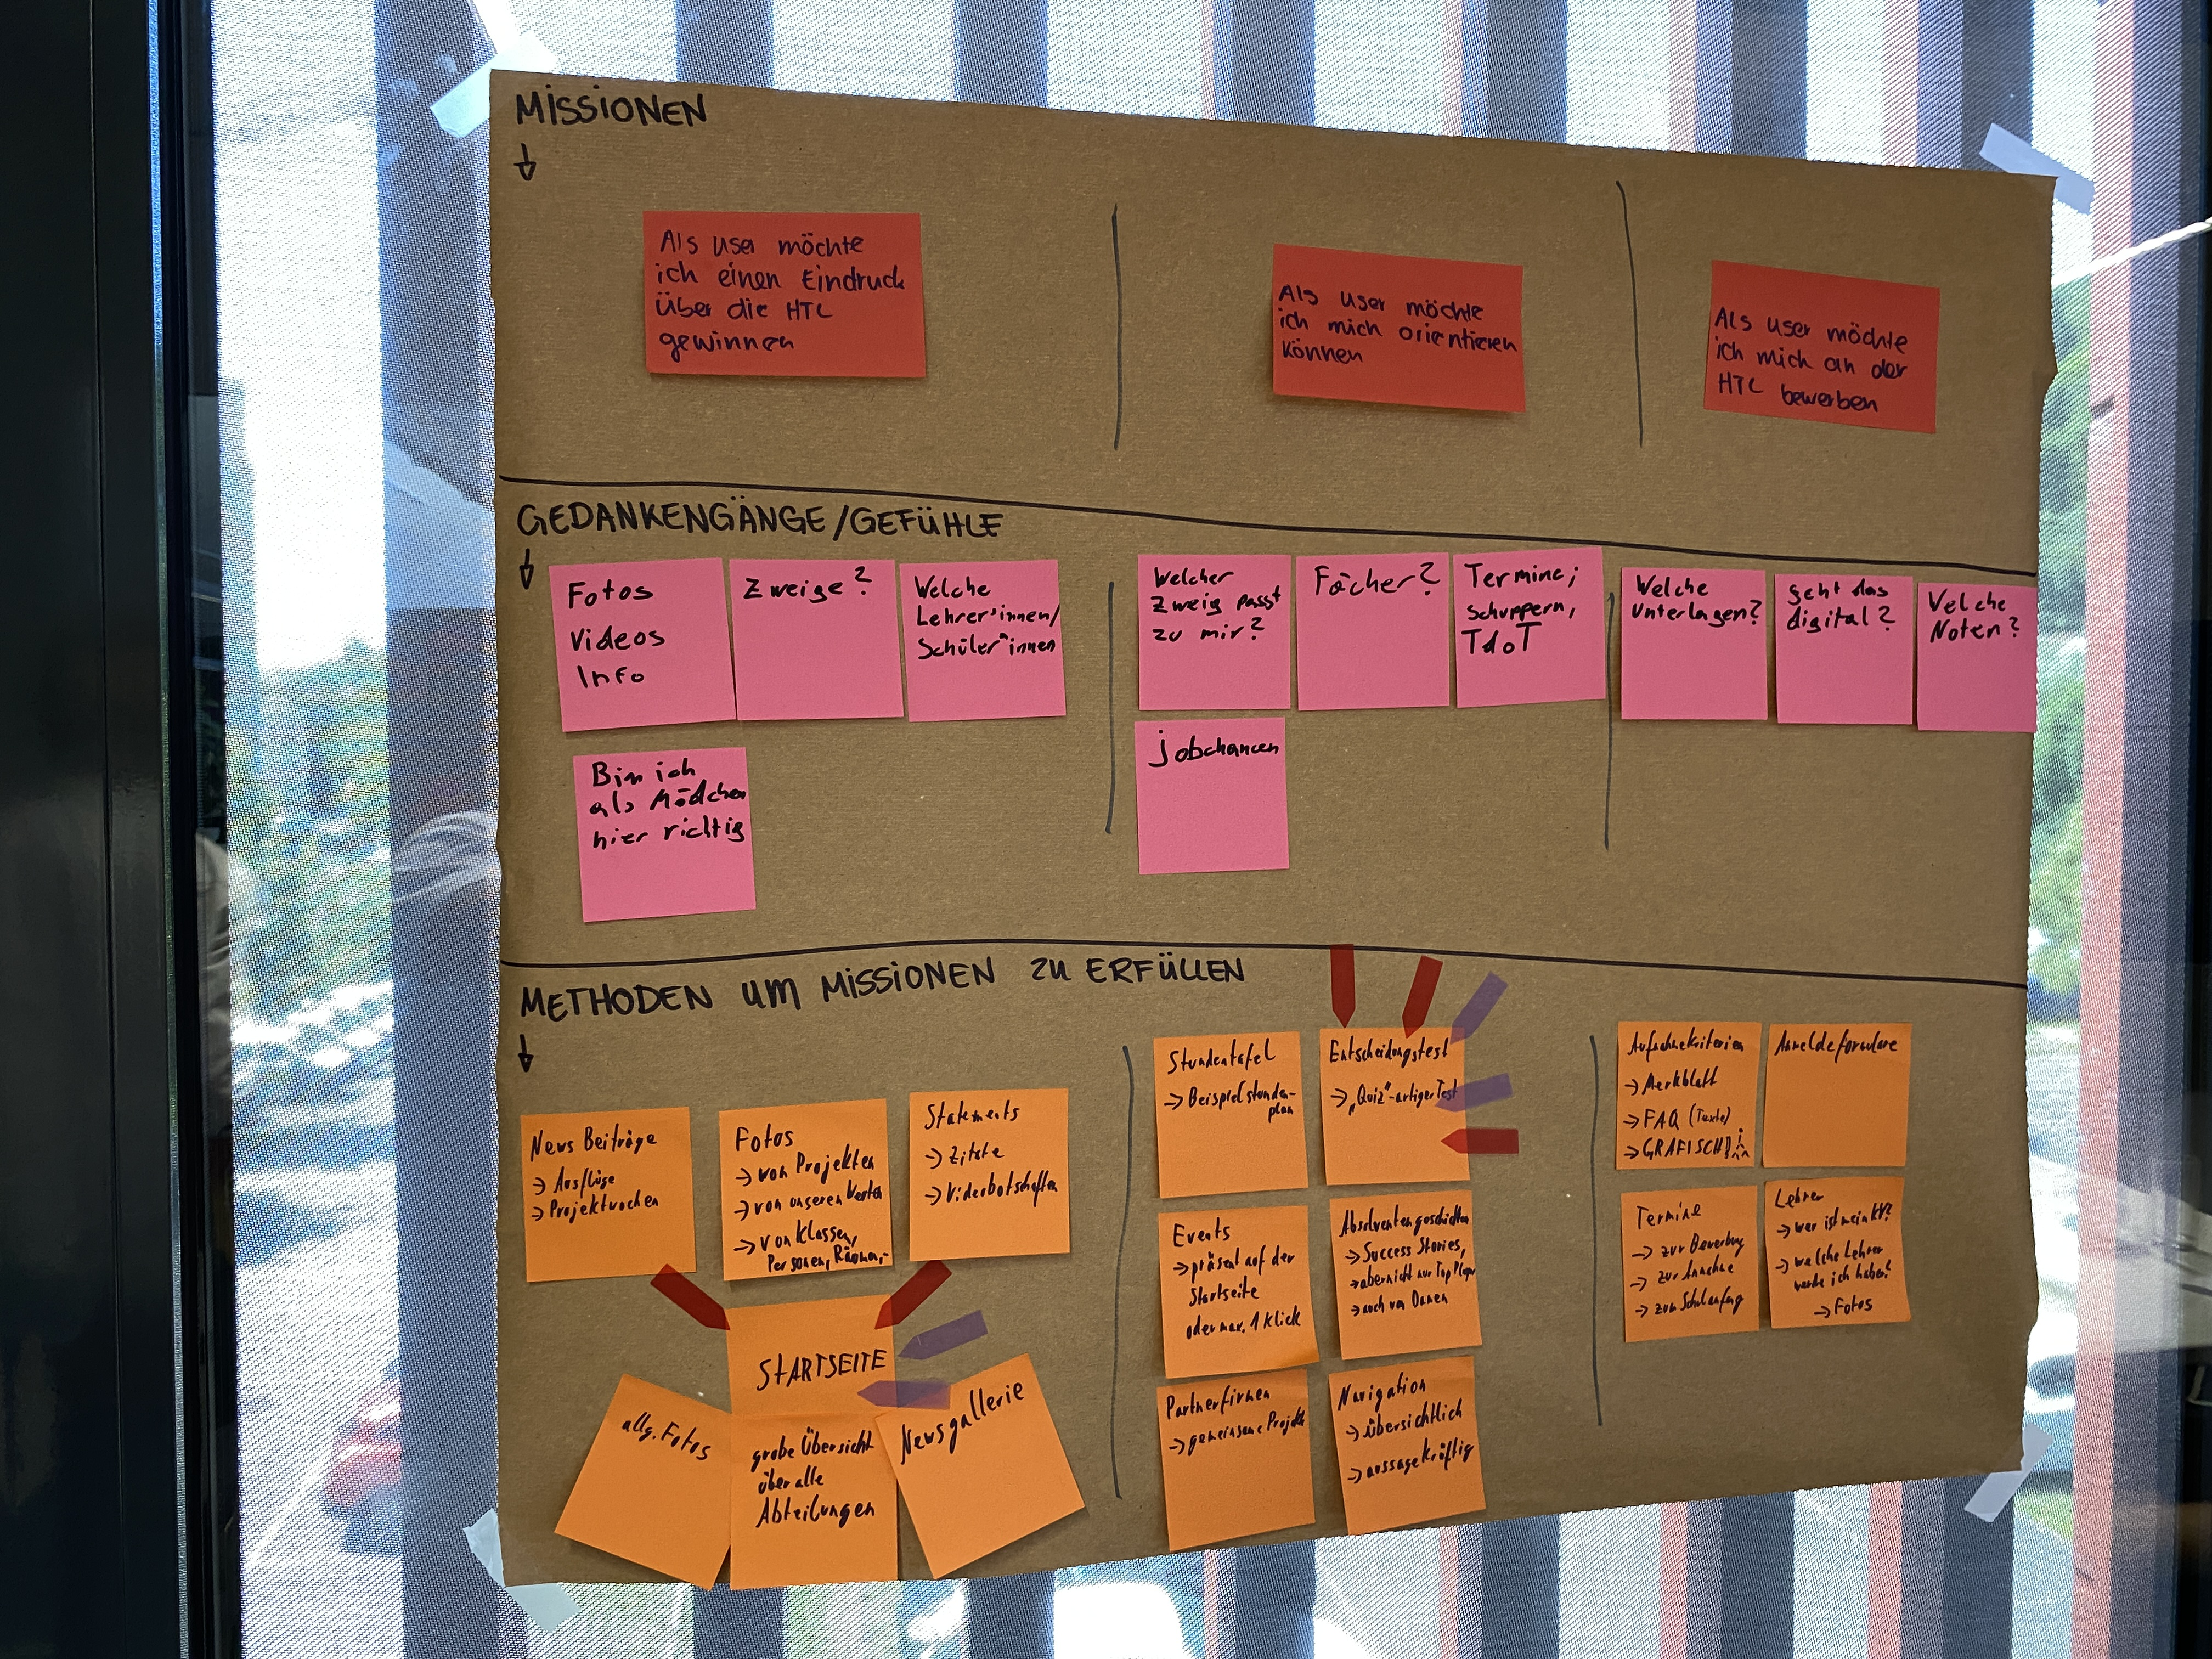
\includegraphics[width=\linewidth]{pics/user_missionen.JPG}
      \caption{UserInnen Missionen}
      \label{fig:impl:user:missionen}
   \end{minipage}
\end{figure}

Um eine intuitive Benutzererfahrung auf der Website sicherzustellen, werden darüber hinaus potenzielle Missionen, 
Gedankengänge und Vorgehensweisen der NutzerInnen berücksichtigt, die sie bei ihrem Besuch auf dem HTL-Webauftritt haben könnten (Siehe Abbildung \ref{fig:impl:user:missionen}). 
Es wurde dabei analysiert, welche konkreten Ziele sie verfolgen, welche Informationen sie suchen und welche Schritte sie wahrscheinlich unternehmen möchten.

Diese detaillierte Betrachtung der Nutzerinteraktion ermöglicht es, die Benutzeroberfläche so zu gestalten, dass sie den natürlichen Denk- und Handlungsmustern 
der BenutzerInnen entspricht. Durch das Verstehen der potenziellen Missionen und Gedankengänge wird sichergestellt, dass die Website nicht nur informativ ist, 
sondern auch nahtlos in den individuellen Ablauf der NutzerInnen integriert wird. Dieser Ansatz fördert eine reibungslose und effektive Nutzung der Website.

Mit dem erlangten Wissen über die zu behebenden Probleme und die unterschiedlichen Usergruppen, deren individuelle Anforderungen 
an die HTL-Website, die Ziele, die sie mit dem Besuch der Website verfolgen möchten und die Emotionen und Eindrücke, die man in den Usern beim benutzen der Oberfläche erwecken will,
wird nun der Startpunkt für die Erstellung eines Designentwurfs erleichtert. Dazu wurde unter den
TeilnehmerInnen des Workshops Zettel und Stifte ausgeteilt, um Skizzen und mögliche Layouts für die Weboberfläche zu gestalten. (Siehe Abbildung \ref{fig:impl:erste_entwuerfe})
Durch diese Methode werden eine Vielzahl an Ideen erbracht, die in der gesamten Gruppe geteilt und diskutiert werden. 
Dieser kreative Ansatz ermöglicht es, die gewonnenen Erkenntnisse 
unmittelbar in konkrete visuelle Konzepte umzusetzen und so den Grundstein für eine optimierte HTL-Website zu legen.

\begin{figure}
   \centering
   \begin{subfigure}{0.3\textwidth}
     \includegraphics[width=\textwidth, angle=270]{pics/Entwurf_Beispiel_1.JPG}
     \caption{Entwurf 1}
     \label{fig:a}
   \end{subfigure}
   \hfill
   \begin{subfigure}{0.3\textwidth}
     \includegraphics[width=\textwidth, angle=270]{pics/Entwurf_Beispiel_2.JPG}
     \caption{Entwurf 2}
     \label{fig:b}
   \end{subfigure}
   \hfill
   \begin{subfigure}{0.3\textwidth}
     \includegraphics[width=\textwidth, angle=270]{pics/Entwurf_Beispiel_3.JPG}
     \caption{Entwurf 3}
     \label{fig:c}
   \end{subfigure}
   \caption{erste Entwürfe}
   \label{fig:impl:erste_entwuerfe}
 \end{figure}

\section{Entwurf und Usability-Tests}
\setauthor{Angerer Mona}
Nach umfassenden Analysen und Untersuchungen der geeigneten Gestaltungselemente, Effekte und Animationen für die HTL-Website wird unter Anwendung des im Workshop 
erworbenen Wissens und der Designmethoden ein erster Entwurf erstellt. Die Gestaltung wird mithilfe der Plattform Figma in Form eines 
Click-Dummies skizziert. (Siehe Abbildung \ref{fig:impl:figma_entwurf}) Anschließend präsentiert man diesen Entwurf SchülerInnen der ersten und zweiten Klasse der HTL sowie Lehrkräften 
und externen Personen. Diese Form der Testung ermöglicht es, direktes Feedback und Bewertungen zu sammeln, um den Entwurf 
weiter zu verfeinern und optimal an die Bedürfnisse der BenutzerInnen anzupassen. Der Prozess integriert somit gezielt die Perspektiven 
der verschiedenen Zielgruppen, um eine benutzerfreundliche Website zu gewährleisten. 
Die erhaltenen Rückmeldungen bekräftigen die verbesserte Struktur und die aufgewertete Anordnung durch die Reduzierung der Menüpunkte. 
Zudem wird bestätigt, dass die Navigation auf der Benutzeroberfläche merklich vereinfacht wurde. Allerdings werden auch einige Anregungen 
und Kritiken geäußert, darunter die Empfehlung, vermehrt Schülerfotos einzubinden, um die Website persönlicher zu gestalten. Diese Maßnahme 
soll dazu beitragen, ein einladenderes Bild der HTL Leonding zu vermitteln. Auch werden einige Verschiebungen von Inhalt in andere Menüpunkte 
vorgeschlagen, um eine logischere Anordnung sicherzustellen. 
Nach der Implementierung dieser Verbesserungsvorschläge wird der Prozess mehrfach wiederholt, um das Design weiter zu perfektionieren und 
eine optimale Zufriedenheit aller BenutzerInnen sowie eine intuitive Steuerung der Website zu erreichen. Auch am Tag der offenen Tür an der HTL Leonding
im Jänner 2024 wurden umfangreiche Umfragen und Tests durchgeführt. Besucher, zu denen BewerberInnen und deren Familienmitglieder, SchülerInnen und LehrerInnen 
zählen haben die Homepage probieren können und anschließend einen Umfragebogen, mit dessen Hilfe Aspekte wie Übersichtlichkeit, Design und Wohlbefinden auf der Website
erfasst wurden, ausfüllen können. Auch war auf den Fragebögen Platz für zusätzliches Feedback bereitgestellt, wodurch einige neue Sichtweisen und 
Ideen gefunden wurden.  

\begin{figure}
   \begin{minipage}[b]{\linewidth} 
      \includegraphics[width=\linewidth]{pics/figma.png}
      \caption{Entwurf mit Figma}
      \label{fig:impl:figma_entwurf}
   \end{minipage}
   \hspace{.05\linewidth}
\end{figure}



\section{Finales Design}
\setauthor{Angerer Mona}
Nachdem der Prozess des Usability-Testings und der Überarbeitungen einige Male durchlaufen
wird, entsteht am Ende ein optimiertes und finales Design. 

Dieses beinhaltet folgende Designelemente und unterscheidet sich in diesen Punkten zu der Gestaltung der bisherigen HTL-Website:


\subsection{Benutzerfreundlichkeit}
\setauthor{Angerer Mona}
Ein wesentlicher Aspekt jeder Hompage sollte die Benutzerfreundlichkeit sein, da sie bestimmt, wie gerne und lange die User die Website bedienen.   
Im Vergleich zum alten Menu-Header (Siehe Abbildung \ref{fig:impl:header:alt}) hat der Neue (Siehe Abbildung \ref{fig:impl:header:neu}) statt 7 nur mehr 5 Elemente, um eine sauberere
   Ansicht zu schaffen und Verwirrung in der Navigation zu vermeiden. Die Inhalte aus dem Reiter \glqq News\grqq{} können nun durch einen Link auf der Seite
   \glqq Über uns\glqq{} erreicht werden, die Partnerfirmen stehen nun auf der Startseite. Der Menüpunkt \glqq Schüler:innen\grqq{} ist nun
   aum rechten Bildschirmrand platziert, um die Hauptelemente des Headers erneut zu vermindern und um eine Art \glqq Profil\grqq{}
   oder \glqq Einloggen\glqq{} zu suggestieren. Dort finden sich ebenfalls keine nur für bereits an der HTL Leonding
   lernende Personen, denn dieser Inhalt wurde umfassend in das LeoWiki ausgelagert. Stattdessen findet man unter 
   dem Reiter jetzt die an der Schule angebotenen Programme und SchülerInnenfotos, um einen persönlichen Einblick zu bieten und 
   den Wünschen und Vorschlägen der bei den Usability-Tests befragten Personen nachzugehen.

\begin{figure}
      \centering
      \includegraphics[scale=0.3]{pics/header_alt.png}
      \caption{alter Header}
      \label{fig:impl:header:alt}
  \end{figure}

  \begin{figure}
   \centering
   \includegraphics[scale=0.3]{pics/header_neu.png}
   \caption{neuer Header}
   \label{fig:impl:header:neu}
\end{figure}

Um die riesige Stundentafel, die derzeit die Fächer und Stundenanzahl in den verschiedenen Jahrgängen aufzeigt zu komprimieren und 
lesbarer und ansprechender zu gestalten, wurde in der Neuimplementierung der Website auch der interaktive Stundenplan eingeführt. Dieser beschreibt nicht nur
die Daten die in der Stundentafel gezeigt werden, sondern vereint in sich auch noch die Fächerbeschreibungen. 

Es wurde für jede Abteilung ein fiktiver Stundenplan erstellt, in dem alle Fächer aller Jahrgänge enthalten sind. Dies entspricht natürlich nicht 
der Realität einer Schulwoche an der HTL Leonding, ermöglicht aber eine ansprechende Gestaltung und einfache Bedienung. Wenn man auf ein Fach des Stundenplans klickt,
wird daneben (oder auf Mobile-Geräten darunter) eine detaillierte Beschreibung des Unterrichtsgegenstandes und eine Tabelle, die zeigt wie viele
Stunden des ausgewählten Faches in jedem Jahrgang enthalten sind, geboten. 
Auch wird um die englischsprachigen SchülerInnen und Benutzer anzusprechen im Menuheader die Möglichkeit eines einfachen
Wechsels von Deutsch auf Englisch angeboten. Dies erfolgt über ein Icon welches eine Weltkugel symbolisiert und daneben das Kürzel der
Sprache anzeigt, zu der man mittels eines einfachen Klicks wechseln kann. 


\begin{figure}
   \begin{minipage}[b]{\linewidth} 
      \includegraphics[scale=0.3]{pics/interaktiver-stundenplan.png}
      \caption{interaktiver Stundenplan IT-Medientechnik}
      \label{fig:impl:interaktiver-stundenplan}
   \end{minipage}
   \hspace{.05\linewidth}
\end{figure}

\subsection{Farben und Formen}
\setauthor{Angerer Mona}
Da die bisherige Website sehr viele Farben beinhaltete, erschien sie überladen und überfordernd, was Benutzer potenziell abschreckt, da sie durch die 
vielen visuellen Reize, die ihr Hirn empfängt, nicht wissen, wohin sie klicken oder scrollen sollen um die von ihnen gewünschte Information zu finden.
Nun wird bei der Gestaltung auf viel weiße Fläche gesetzt, die abgesehen von dem Bildmaterial lediglich von kleinen Akzenten 
in den vier Farben der Abteilungen, die auch im Logo vorkommen, und einer fünften Farbe, die eine Mischung der vier 
"HTL-Leonding-Farben" ist, unterbrochen wird. Der Trend zu viel "Whitespace" ist, wie im Kapiel \nameref{sec:Recherche} bereits
behandelt wurde, ein häufig aufkommendes, modernes Designkonzept.

Auch wurde statt auf das starre Block-Design auf mehr Abwechslung und Bewegung in den Formen gesetzt.
So ist das Dreieck eine der wichtigsten Elemente des neuen Webauftritts. Der Grund, weshalt die Wahl 
auf ausgerechnet diese Grundform gefallen ist, liegt in dem Logo der Schule. Dieses besteht aus einem Pfeil,
in dem sich die bereits angesprochenen vier Abteilungsfarben wiederspiegeln. Mittels der verschiedenen
implementierung des Dreiecks auf den unterschiedlichen Seiten der Website finden sich so die Schrägen,
die man bereits im Logo findet, wieder und stärkt somit das gesamte Branding und das Look and Feel der HTL-Website. Auch erscheint der Gesamteindruck
dynamischer und spannender, was zu einer verbesserten User-Experience führt.

\begin{figure}
   \begin{minipage}[b]{\linewidth} 
      \includegraphics[scale=0.3]{pics/Farbpalette.png}
      \caption{Farbpalette HTL Leonding}
      \label{fig:impl:Farbpalette}
   \end{minipage}
   \hspace{.05\linewidth}
\end{figure}

\subsection{Dynamik und Bewegung}
\setauthor{Angerer Mona}
Die wiederholte Verwendung des nicht-typischen, wandelbaren Elements des Dreiecks ist nicht nur dazu da, um visuelle Interesse zu wecken, 
sondern auch, um Spannung und Dynamik in die Weboberfläche zu bringen. Die einzigartige Form des Dreiecks wird oft als visuelles Highlight 
eingesetzt, das die Aufmerksamkeit der Benutzer auf sich zieht und eine gewisse Energie und Bewegung in das Design einbringt. 
Diese dynamischen Elemente tragen dazu bei, dass die Website lebendig und ansprechend wirkt, was wiederum die Benutzererfahrung verbessert.

Darüber hinaus sind viele sich bewegende Objekte in das Design der Website integriert, um eine zusätzliche Dimension von Interaktivität 
und Engagement zu schaffen. Diese bewegten Inhalte werden jedoch mit Bedacht eingesetzt, um keine Unruhe oder Stress bei den Benutzern 
auszulösen. Sie sind subtil und dezent animiert, und ihre Bewegungen sind langsam und fließend, um ein angenehmes und harmonisches 
Nutzererlebnis zu gewährleisten.

Ein Beispiel für diese subtile Bewegung findet sich auf der Seite "Abteilungen", wo eine Übersicht der Fächernamen von links nach rechts 
und umgekehrt über den Bildschirm gleitet. Diese sanfte Bewegung verleiht der Seite eine gewisse Lebendigkeit, ohne dabei ablenkend oder 
überwältigend zu wirken. Ähnlich ist es auf den Seiten der einzelnen Abteilungen, wie beispielsweise "Informatik - SSE", wo eine Reihe von
 Bildern, die die Fachrichtung beschreiben, sich vertikal über das Display bewegt. Diese dezente Animation trägt dazu bei, dass die Seite dynamisch und ansprechend wirkt, ohne dabei die Benutzer abzulenken oder zu überfordern.

Diese Animationen und bewegten Objekte sind ein effektives Mittel, um die Benutzerinteraktion zu verbessern und das
 Design der Website lebendig und ansprechend zu gestalten. Durch ihre geschickte Integration in das Gesamtkonzept der Website tragen sie 
 dazu bei, eine positive und einprägsame Benutzererfahrung zu schaffen, die die Markenwahrnehmung stärkt und die Besucher dazu ermutigt, 
 sich länger auf der Seite aufzuhalten.


\subsection{Grafiken und Animationen}
\setauthor{Angerer Mona}
In der Gestaltung der Website wurde bewusst der Einsatz von Animationen und grafischen Elementen gewählt, 
um das schlichte Design, welches durch den großzügigen Einsatz von Whitespace entstanden ist, gezielt aufzulockern und 
zu bereichern. Durch das Hinzufügen der Startanimation beim Laden der Website sowie individuellen Animationen für jede 
Abteilung der Schule wird eine dynamische und ansprechende Benutzererfahrung geschaffen. Ergänzend dazu wurden gezielte Grafiken und 
Illustrationen eingeführt, die nicht nur ästhetisch ansprechend sind, sondern auch dazu dienen, Informationen visuell 
darzustellen und den Inhalt der Website aufzuwerten.

Diese Animationen und Grafiken dienen nicht nur der reinen Ästhetik, sondern haben auch funktionale Aspekte. 
Sie führen den Benutzer intuitiv durch die Website, lenken die Aufmerksamkeit auf wichtige Informationen und verbessern die 
Usability. Darüber hinaus tragen sie dazu bei, die Identität und das Branding der HTL-Website zu stärken, indem sie ein 
kohärentes und durchdachtes Benutzererlebnis bieten.

Durch die Integration von animierten Grafiken und visuellen Elementen wird das Engagement der Benutzer erhöht und ein 
interaktiveres Erlebnis geschaffen. Die sorgfältig ausgewählten Grafiken unterstützen die Inhalte der Website, machen diese 
zugänglicher und erleichtern das Verständnis komplexer Themen. Insgesamt unterstützen die Animationen und Grafiken das Ziel der Homepage, 
den Besuchern einen informativen, ansprechenden und nahtlosen Zugang zu den verschiedenen Abteilungen und Inhalten zu ermöglichen, 
während sie gleichzeitig das Markenimage der HTL stärken.

\begin{figure}
   \begin{minipage}[b]{.4\linewidth} 
      \includegraphics[width=\linewidth]{pics/grafik-start.png}
      \caption{Grafik der Startseite}
      \label{fig:impl:grafik:start}
   \end{minipage}
   \hspace{.05\linewidth}
   \begin{minipage}[b]{.4\linewidth}
      \includegraphics[width=\linewidth]{pics/grafik-ausbildung.png}
      \caption{Grafik der Ausbildungsseite}
      \label{fig:impl:grafik:ausbildung}
   \end{minipage}
\end{figure}


\subsection{Dark Mode}
\setauthor{Angerer Mona}

Für eine benutzerfreundliche und adaptive Website-Erfahrung wurde die Implementierung eines Dark Modes vorgenommen, 
der sich automatisch an die Computereinstellungen des Nutzers anpasst. Diese Funktion berücksichtigt die systemweiten Einstellungen 
des Benutzers und schaltet automatisch zwischen dem hellen und dem dunklen Modus um, je nachdem, welche Einstellung auf dem jeweiligen 
Gerät aktiviert ist. Dies unterscheidet sich maßgeblich von der aktuellen HTL-Homepage, auf der der Dark-Mode auf der Weboberfläche manuell
an- oder ausgestellt werden musste. Durch diese Anpassungsfähigkeit wird nicht nur die Lesbarkeit und der visuelle Komfort für den Benutzer 
verbessert, sondern es wird auch ein nahtloses und konsistentes Benutzererlebnis über verschiedene Geräte und Plattformen hinweg 
gewährleistet. Diese automatische Anpassung des Dark Modes an die individuellen Computereinstellungen reflektiert die Bestrebungen, 
die Website so benutzerzentriert und zugänglich wie möglich zu gestalten, indem sie den persönlichen Vorlieben und Bedürfnissen der
Nutzer gerecht wird.

\begin{figure}
   \begin{minipage}[b]{\linewidth} 
      \includegraphics[scale=0.3]{pics/Example_Darkmode.png}
      \caption{Beispiel Dark-Mode}
      \label{fig:impl:example_darkmode}
   \end{minipage}
   \hspace{.05\linewidth}
\end{figure}


\subsection{Kontinuierliches Design}
\setauthor{Angerer Mona}

Einer der fundamentalsten Aspekte beim Entwickeln eines Designs ist der sogenannte rote Faden, der sich durch das Look and Feel der gesamten
Website ziehen soll. Ein kohärentes Design hilft, einen Widererkennungswert zu schaffen und das individuelle Branding, in diesem Fall der HTL Leonding,
zu stärken. Alle bereits beschriebenen Punkte tragen im dem Fall der neuen HTl-Homepage zählen dazu bei, unter anderem die distinktiven Dreiecke, die
die Headerelemente der Unterseiten prägen, sowie auch an manchen anderen Stellen Designelemente bilden. Auch die bereits beschreiebenen
einheitlichen Farben, die sowohl im Logo als auch in alle anderen farblichen Elementen vorkommen, prägen das individuelle Branding der Website.
Es wird auch darauf geachtet, dass alle Hover-Effekte sowie Links (zum Beispiel auf der Ausbildungsseite (Siehe Abbildung \ref{fig:impl:link:ausbildung}) oder
 im Newsroom (Siehe Abbildung \ref{fig:impl:link:news})) beständig und identisch gestaltet sind.
\begin{figure}
   \begin{minipage}[b]{.4\linewidth} 
      \includegraphics[width=\linewidth]{pics/beispiel links ausbildung.png}
      \caption{Links auf der Ausbildungsseite}
      \label{fig:impl:link:ausbildung}
   \end{minipage}
   \hspace{.05\linewidth}
   \begin{minipage}[b]{.4\linewidth}
      \includegraphics[width=\linewidth]{pics/beispiel links newsroom.png}
      \caption{Link auf der Newsroom-Seite}
      \label{fig:impl:link:news}
   \end{minipage}
\end{figure}

\subsection{Schriftart}
\setauthor{Angerer Mona}

Die Entscheidung, bei der Gestaltung des neuen Webauftritts der HTL Leonding weiterhin auf die Schriftart 'Manrope' zu setzen, 
ist das Ergebnis einer gründlichen Analyse und Abwägung verschiedener Faktoren. 'Manrope' wurde bereits auf der bisherigen HTL-Website 
implementiert und hat sich als eine äußerst geeignete Wahl erwiesen, die sowohl ästhetische als auch funktionale Anforderungen erfüllt.

Eine der wichtigsten Eigenschaften von 'Manrope' ist ihre Vielseitigkeit und Lesbarkeit. Diese Schriftart zeichnet sich durch klare Linien, 
gut definierte Buchstabenformen und eine angenehme Lesbarkeit aus, die sie zu einer idealen Wahl für den Einsatz in digitalen Medien macht. 
Die klare und gut lesbare Schrift verbessert die Benutzererfahrung und erleichtert es den Besuchern, den angebotenen Inhalt schnell und 
einfach zu erfassen.

Darüber hinaus verleiht 'Manrope' dem Design eine moderne und professionelle Ästhetik. Die klaren Linien und die ausgewogene Proportionierung 
verleihen der Schrift einen zeitgemäßen Look, der sich perfekt in ein modernes Webdesign einfügt. Dies trägt dazu bei, dass der neue Webauftritt 
der HTL Leonding ein ansprechendes und zeitgemäßes Erscheinungsbild hat, das das Image der Schule als innovative Bildungseinrichtung unterstreicht.

Auch zeichnet sich diese Schriftart über ihre Verfügbarkeit und Anpassbarkeit aus. 'Manrope' ist in verschiedenen Schnitten und 
Stilen erhältlich, was es ermöglicht, sie flexibel und vielseitig einzusetzen. Von leichten bis zu fetten Schnitten bietet 
'Manrope' eine breite Palette von Optionen, die es den Designern ermöglichen, die Schrift je nach Kontext und Anforderungen des Designs 
anzupassen.
'Manrope' bietet ebenfalls eine gute Lesbarkeit auf verschiedenen Bildschirmgrößen und Gerätetypen. Diese Schriftart wurde 
speziell für den Einsatz in digitalen Medien optimiert und gewährleistet eine konsistente Darstellung und Lesbarkeit auf allen Geräten, 
einschließlich Desktop-Computern, Laptops, Tablets und Smartphones.

Verschiedene Verwendungen der Schriftart in verschiedenen Schriftschnitten sind beispielsweise die Headerüberschriften (Siehe Abbildung \ref{fig:man:b}), 
die Unterüberschriften, hier Beispielsweise auf der Startseite (Siehe Abbildung \ref{fig:man:a}) oder im Fließtext (Siehe Abbildung \ref{fig:man:c}).

\begin{figure}
   \begin{minipage}[b]{\linewidth} 
      \includegraphics[scale=0.3]{pics/manrope.png}
      \caption{Manrope}
      \label{fig:impl:manrope}
   \end{minipage}
   \hspace{.05\linewidth}
\end{figure}

\begin{figure}
   \centering
   \begin{subfigure}{0.3\textwidth}
     \includegraphics[width=\textwidth]{pics/manrope1.png}
     \caption{Unterüberschrift}
     \label{fig:man:a}
   \end{subfigure}
   \hfill
   \begin{subfigure}{0.3\textwidth}
     \includegraphics[width=\textwidth]{pics/manrope2.png}
     \caption{Header}
     \label{fig:man:b}
   \end{subfigure}
   \hfill
   \begin{subfigure}{0.3\textwidth}
     \includegraphics[width=\textwidth]{pics/manrope3.png}
     \caption{Entwurf 3}
     \label{fig:man:c}
   \end{subfigure}
   \caption{Fließtext}
   \label{fig:impl:erste_entwuerfe}
 \end{figure}


\section{Aufbau und Unterseiten}
\setauthor{Angerer Mona}


\subsection{Startseite}
\setauthor{Angerer Mona}

Wenn man die neue HTL Leonding-Website aufruft, wird zuallererst eine kurze Animation gezeigt, die die Aufmerksamkeit des Benutzers ab des 
ersten Moments voll und ganz auf sich zieht. Nach dem spannenden Einstieg werden anschließend die wichtigsten News-Beiträge gezeigt, um vor allem
den BererberInnen und Elternteilen den aufregenden und abwechlungsreichen Schulalltag zu beschreiben. Ein kleiner Pfeil am unteren Bildschrimrand,
der aus dem um 90 Grad gedrehten Schullogo besteht, symbolisiert dem User dass man um den restlichen Content zu sehen nach unten scrollen muss. Die restlichen
News-Beiträge scrollen horizontal von dem rechten Bildschirmrand hinein und neuer Content der Seite wird sichtbar. Dieser besteht aus den sogenannten 
"featured events", die aus anstehenden Versanstaltungen oder Ereignisse an der HTL Leonding aufzeigt. 
Abschließend läuft ein automatischer horizontaler Scroller, der die Sponsoren und Partner der HTL Leonding, veranschaulichen. Die Einbindung dieser Firmen 
auf der Startseite ersetzt somit die eigene Unterseite 'Partner', die bisher auf der HTL Leonding Website zu finden war.

Die Startseite ist kurz und bündig gehalten, beinhaltet trotzdem viele wichtigen Information zu der HTL Leonding und ebnet den Weg zur weiteren Navigation
durch die Website.

\begin{figure}
   \begin{minipage}[b]{.4\linewidth} 
      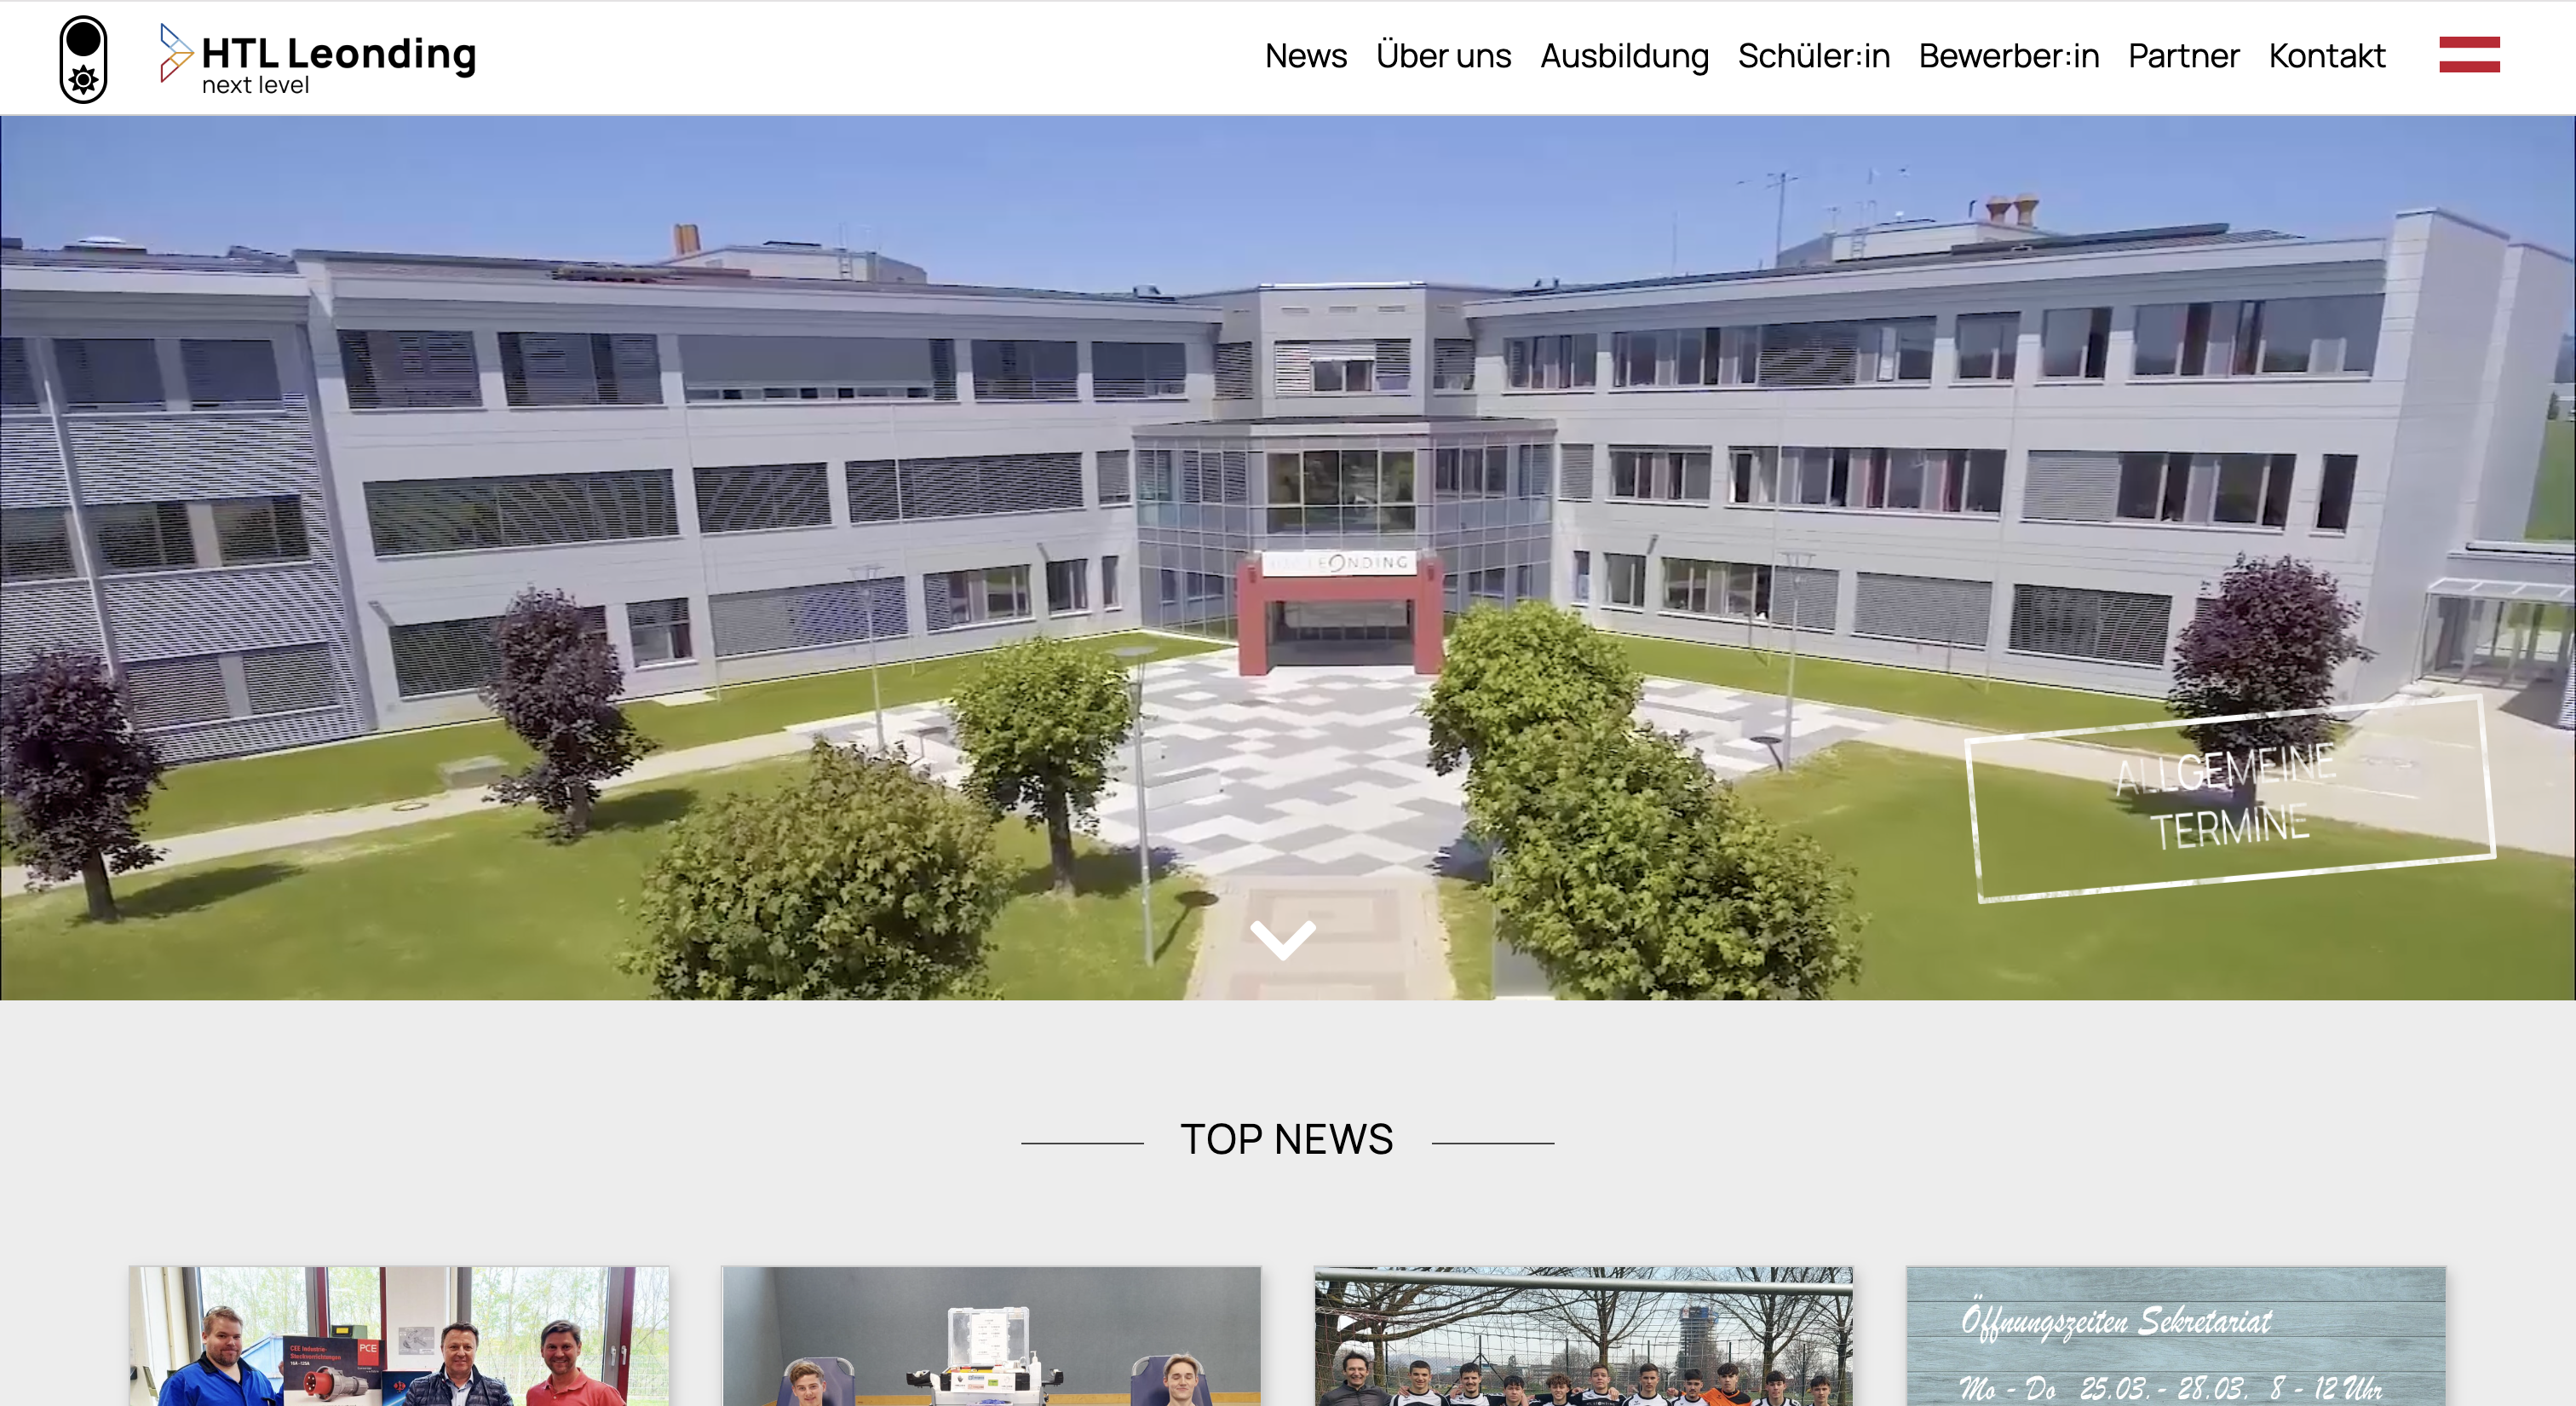
\includegraphics[width=\linewidth]{pics/alt-start.png}
      \caption{alte Startseite}
      \label{fig:impl:alt:start}
   \end{minipage}
   \hspace{.05\linewidth}
   \begin{minipage}[b]{.4\linewidth}
      \includegraphics[width=\linewidth]{pics/neu-start.png}
      \caption{neue Startseite}
      \label{fig:impl:neu:start}
   \end{minipage}
\end{figure}



\subsection{Über uns}
\setauthor{Angerer Mona}

Die 'Über uns'-Seite der HTL Leonding ist eine facettenreiche Darstellung, die zahlreiche prägnante Elemente enthält. 
Bei einem Blick auf die linke Bildschirmseite fällt sofort die charakteristische Dreiecksform auf, 
die sich durch das gesamte Design zieht und einen visuellen Zusammenhalt schafft. Diese Dreiecksform kann symbolisch für die dynamische und 
innovative Atmosphäre der Schule stehen und spiegelt sich auch in den einheitlichen Farben und Links wider, die einen konsistenten Schulauftritt 
gewährleisten.

Trotz der Vielzahl von Inhalten, die auf dieser Seite präsentiert werden, wird auf ausreichend Whitespace geachtet, um ein klares und 
aufgeräumtes Erscheinungsbild zu gewährleisten. Dies ermöglicht den Besuchern, sich auf die präsentierten Informationen zu konzentrieren, 
ohne von einem überladenen Layout abgelenkt zu werden. Das schlichte und ordentliche Design unterstreicht die Professionalität  
der HTL Leonding als Bildungseinrichtung.

Die 'Über uns'-Seite dient als zentraler Anlaufpunkt für die relevantesten Informationen über die Schule. Durch die Integration von 
Videolinks, Foldern und Weiterleitungen zum Newsroom und zur Abteilungsseite bietet sie den Besuchern eine Vielzahl von Möglichkeiten, 
mehr über die Schule, ihr Bildungsangebot und das Schulleben zu erfahren. Diese Vielfalt an Inhalten und Ressourcen trägt dazu bei, das 
breite Spektrum der Aktivitäten und Möglichkeiten der HTL Leonding transparent darzustellen und potenziellen Interessenten einen umfassenden 
Einblick zu bieten.

\begin{figure}
   \begin{minipage}[b]{.4\linewidth} 
      \includegraphics[width=\linewidth]{pics/alt-überuns.png}
      \caption{alte 'Über uns'- Seite}
      \label{fig:impl:alt:überuns}
   \end{minipage}
   \hspace{.05\linewidth}
   \begin{minipage}[b]{.4\linewidth}
      \includegraphics[width=\linewidth]{pics/neu-überuns.png}
      \caption{alte 'Über uns'- Seite}
      \label{fig:impl:neu:überuns}
   \end{minipage}
\end{figure}

\subsection{News Room}
\setauthor{Angerer Mona}

Den News Room kann man über die 'Über uns'-Seite sowie den Newsbeiträgen auf der Startseite erreichen. Auch er kennzeichnet sich durch 
die Schräge am linken Bildschirmrand, die anders als bei den übrigen Unterseiten aber nicht mit dem Rest des Inhalts der Oberfläche wegscrollt,
sondern seinen Platz fest behält während die Newsbeiträge auf der rechten Seite scrollen.
Auch auf der Neuentwicklung des Newsrooms wurde die Filterfunktion implementiert, die bereits auf der bisherigen Website existiert.
Mit ihr kann man die Beiträge nach den verschiedenen Abteilungen, sowie Kategorien wie Sport oder Reisen filtern. Die Beiträge bestehen alle aus Titelbild,
Datum und zugeordneter Kategorie. Wenn man sich nun aufgrund der Überschrift dazu entschließt, einen Beitrag zu lesen, kann man mittels eines Mausklicks
ganz einfach den Beitrag "ausklappen". Es öffnet sich also nicht mehr, so wie bisher, eine neue Seite, sondern die Artikel lassen sich alle beliebig aus- und einklappen,
ohne die Seite des Newsrooms verlassen zu müssen. Dies ermöglicht ein einfaches "durchblättern" der Beiträge und spart den Benutzern die Ladezeit, 
die es bisher gebraucht hat, eine neue Browserseite zu öffnen.

\begin{figure}
   \begin{minipage}[b]{.4\linewidth} 
      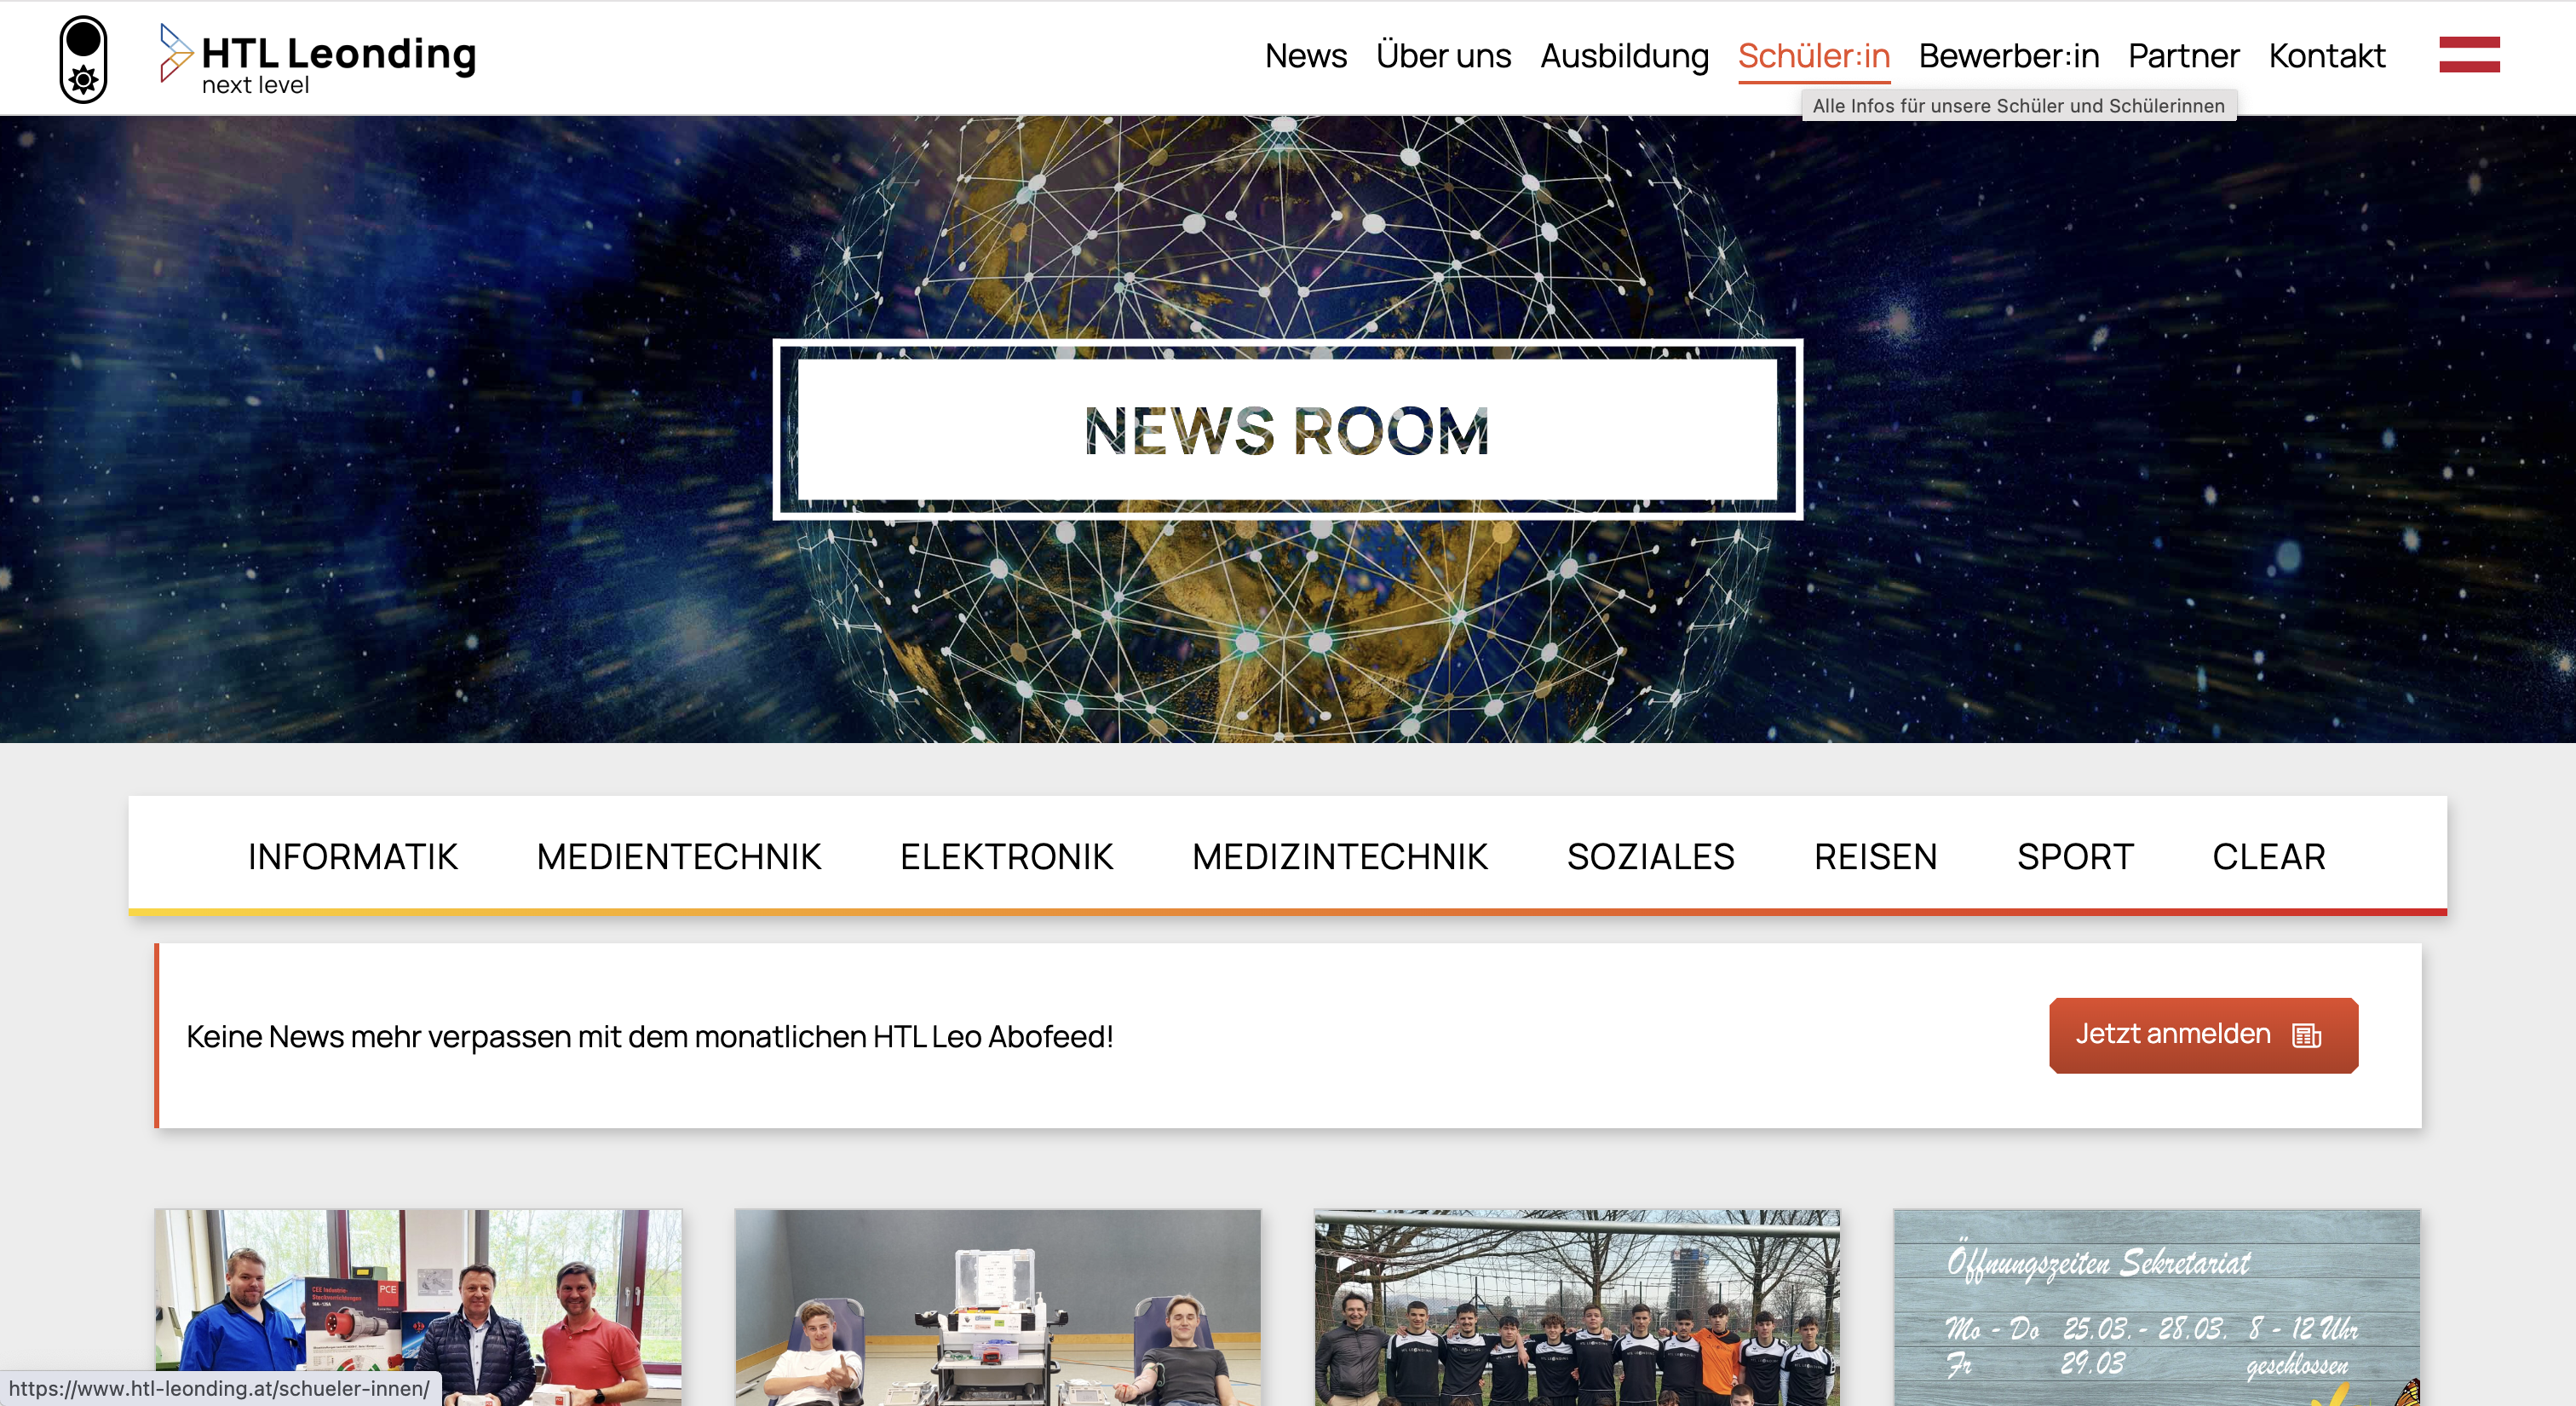
\includegraphics[width=\linewidth]{pics/alt-news.png}
      \caption{alte Newsroomseite}
      \label{fig:impl:alt:start}
   \end{minipage}
   \hspace{.05\linewidth}
   \begin{minipage}[b]{.4\linewidth}
      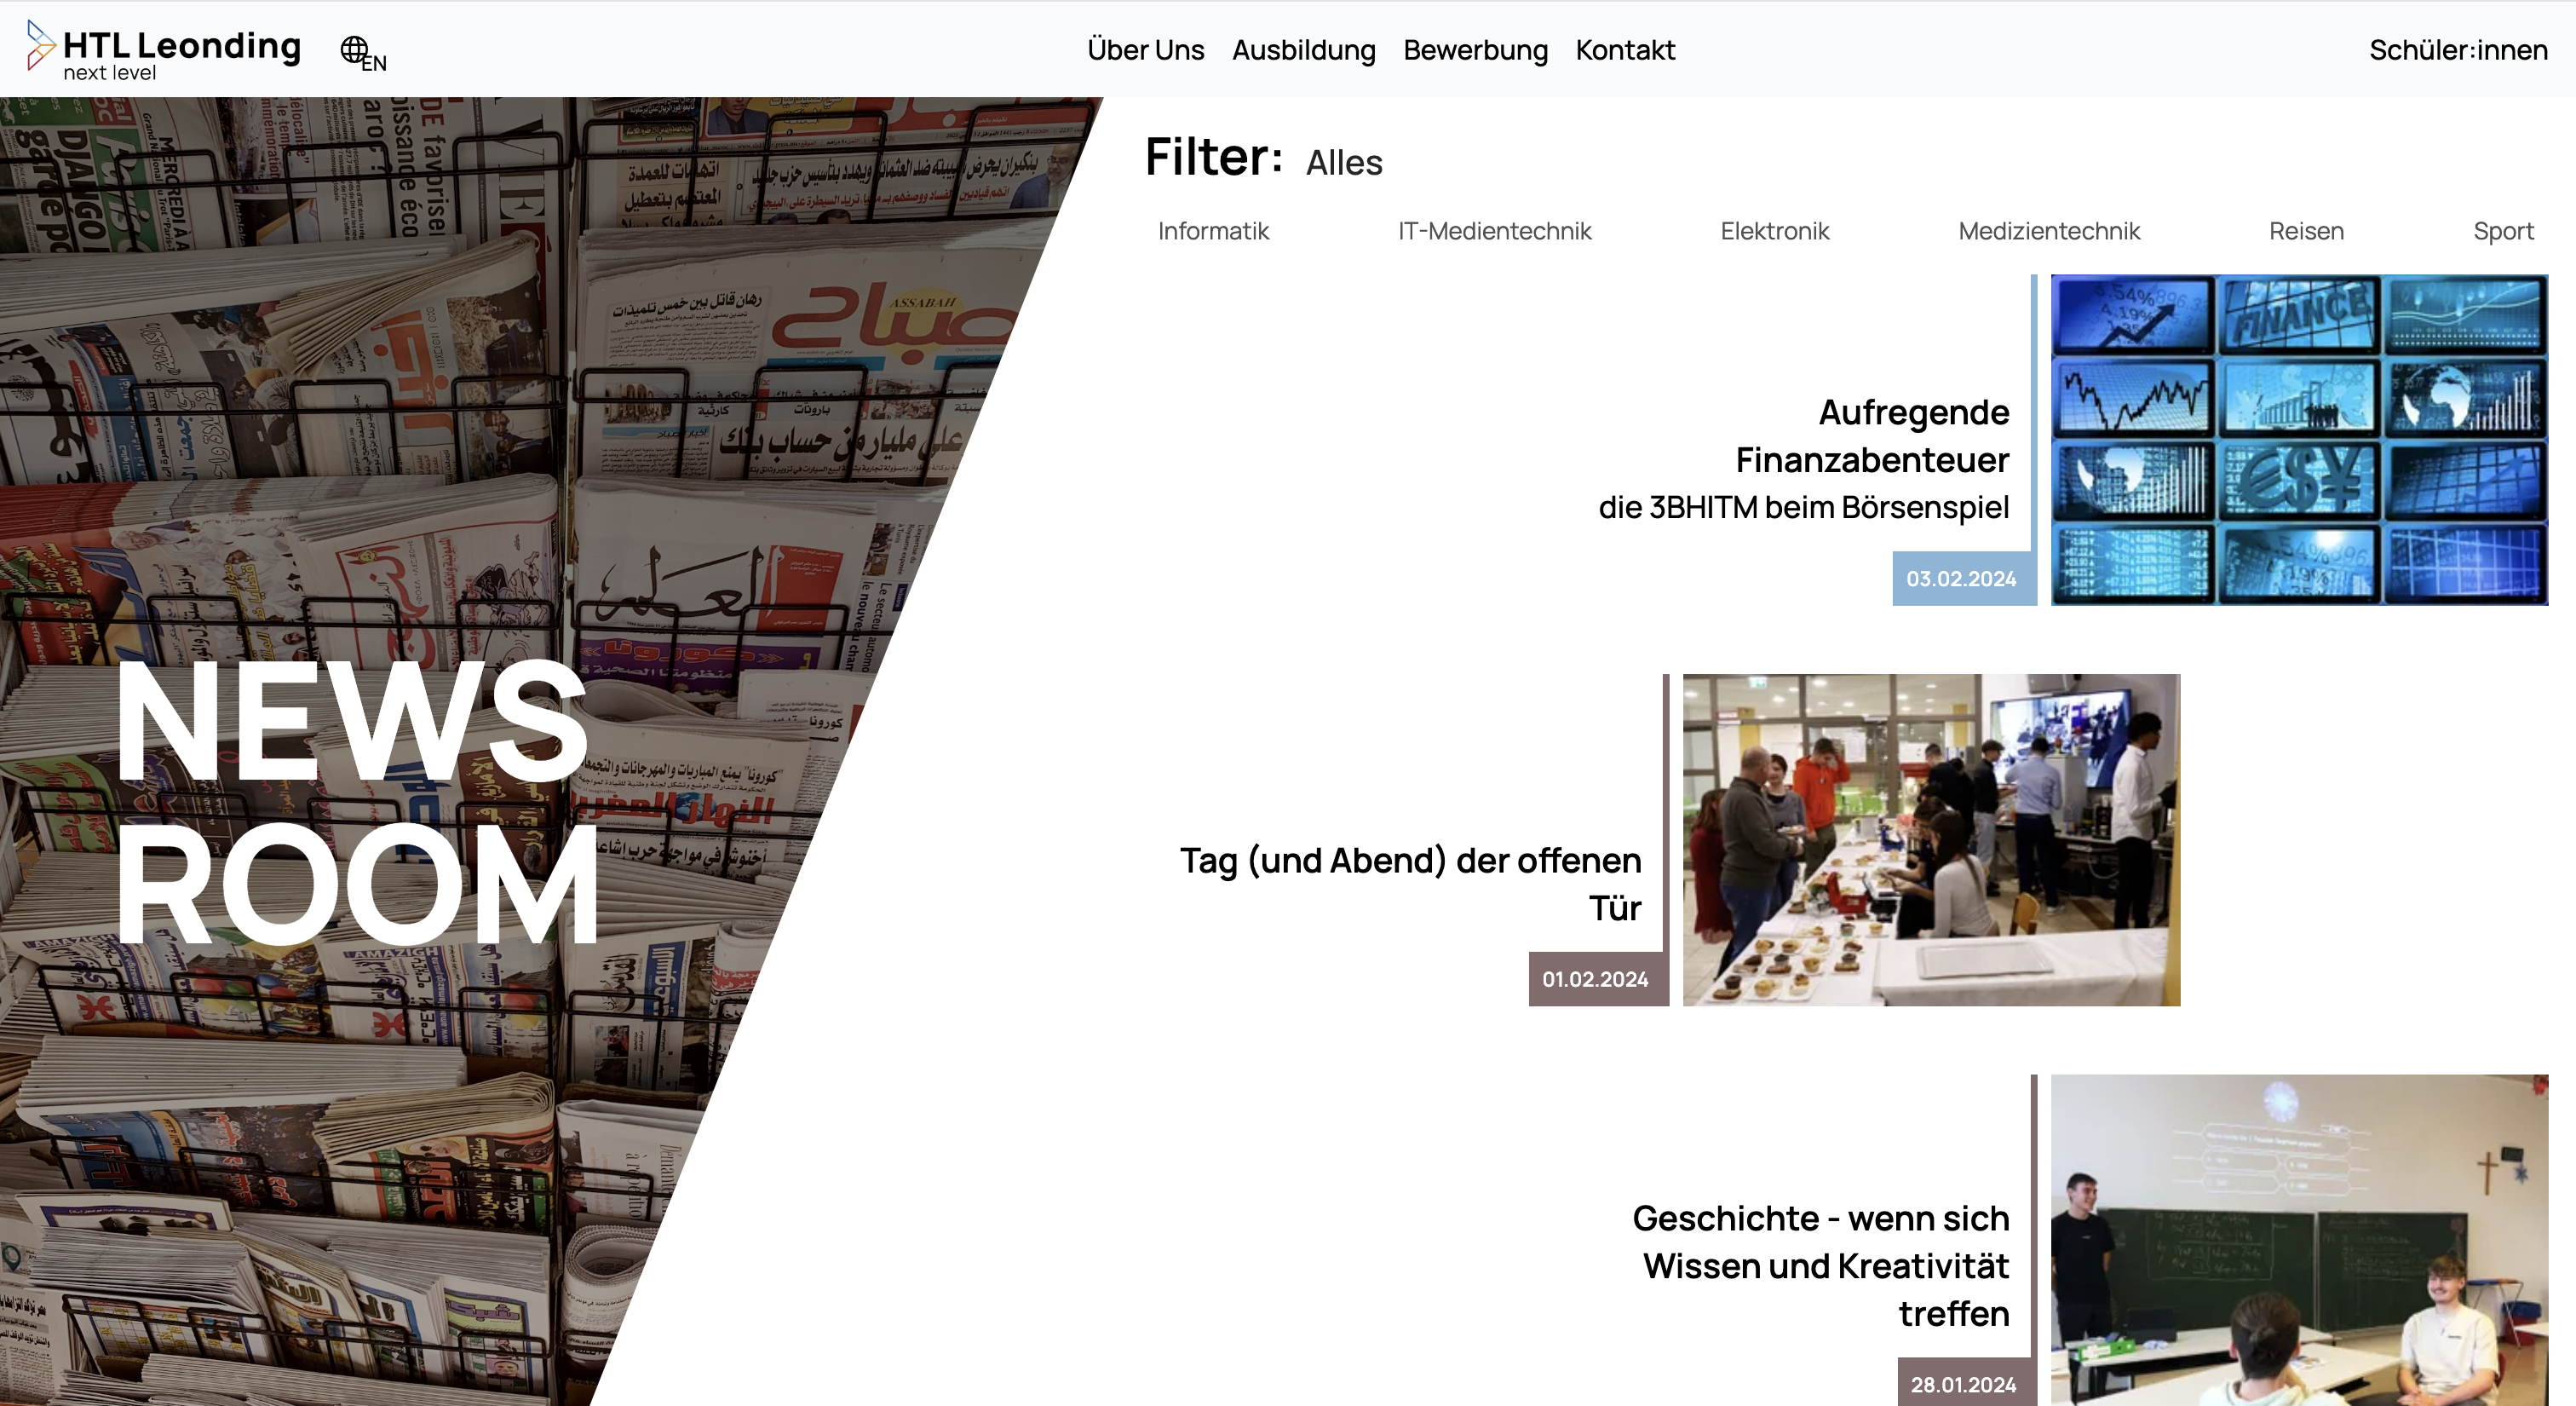
\includegraphics[width=\linewidth]{pics/neu-news.png}
      \caption{neue Newsroomseite}
      \label{fig:impl:neu:start}
   \end{minipage}
   \hspace{.05\linewidth}
   \begin{minipage}[b]{.4\linewidth}
      \includegraphics[width=\linewidth]{pics/neu-newsausgeklappt.png}
      \caption{neue Newsroomseite ausgeklappt}
      \label{fig:impl:neu:start}
   \end{minipage}
\end{figure}

\subsection{Ausbildung}
\setauthor{Angerer Mona}

Da die Ausbildungs-Seite mit zu den wichtigsten einer jeder Schulhomepage gehört, wurde bei der Entwicklung besondere Aufmerksamkeit auf sie gelenkt.
Ebenfalls prägt den oberen Bildschirmrand ein schräg abgeschnittenes Headerbild, zusätzlich verziert mit einer SVG-Grafik des Schulgebäudes.
Nach dem ersten mal scrollen haben die Benutzer beereits alle Ausbildungsmöglichkeiten, die die HTL Leonding bietet, auf einem Blick auf dem Bildschirm.
Simple gestaltete Links zu den jeweiligen Unterseiten zeigen nun anstatt überladener Bilder, wie es bei der bisherigen Website der Fall war, den 
Weg zu den Abteilungen und der Fach- und Abendschule.

\begin{figure}
   \begin{minipage}[b]{.4\linewidth} 
      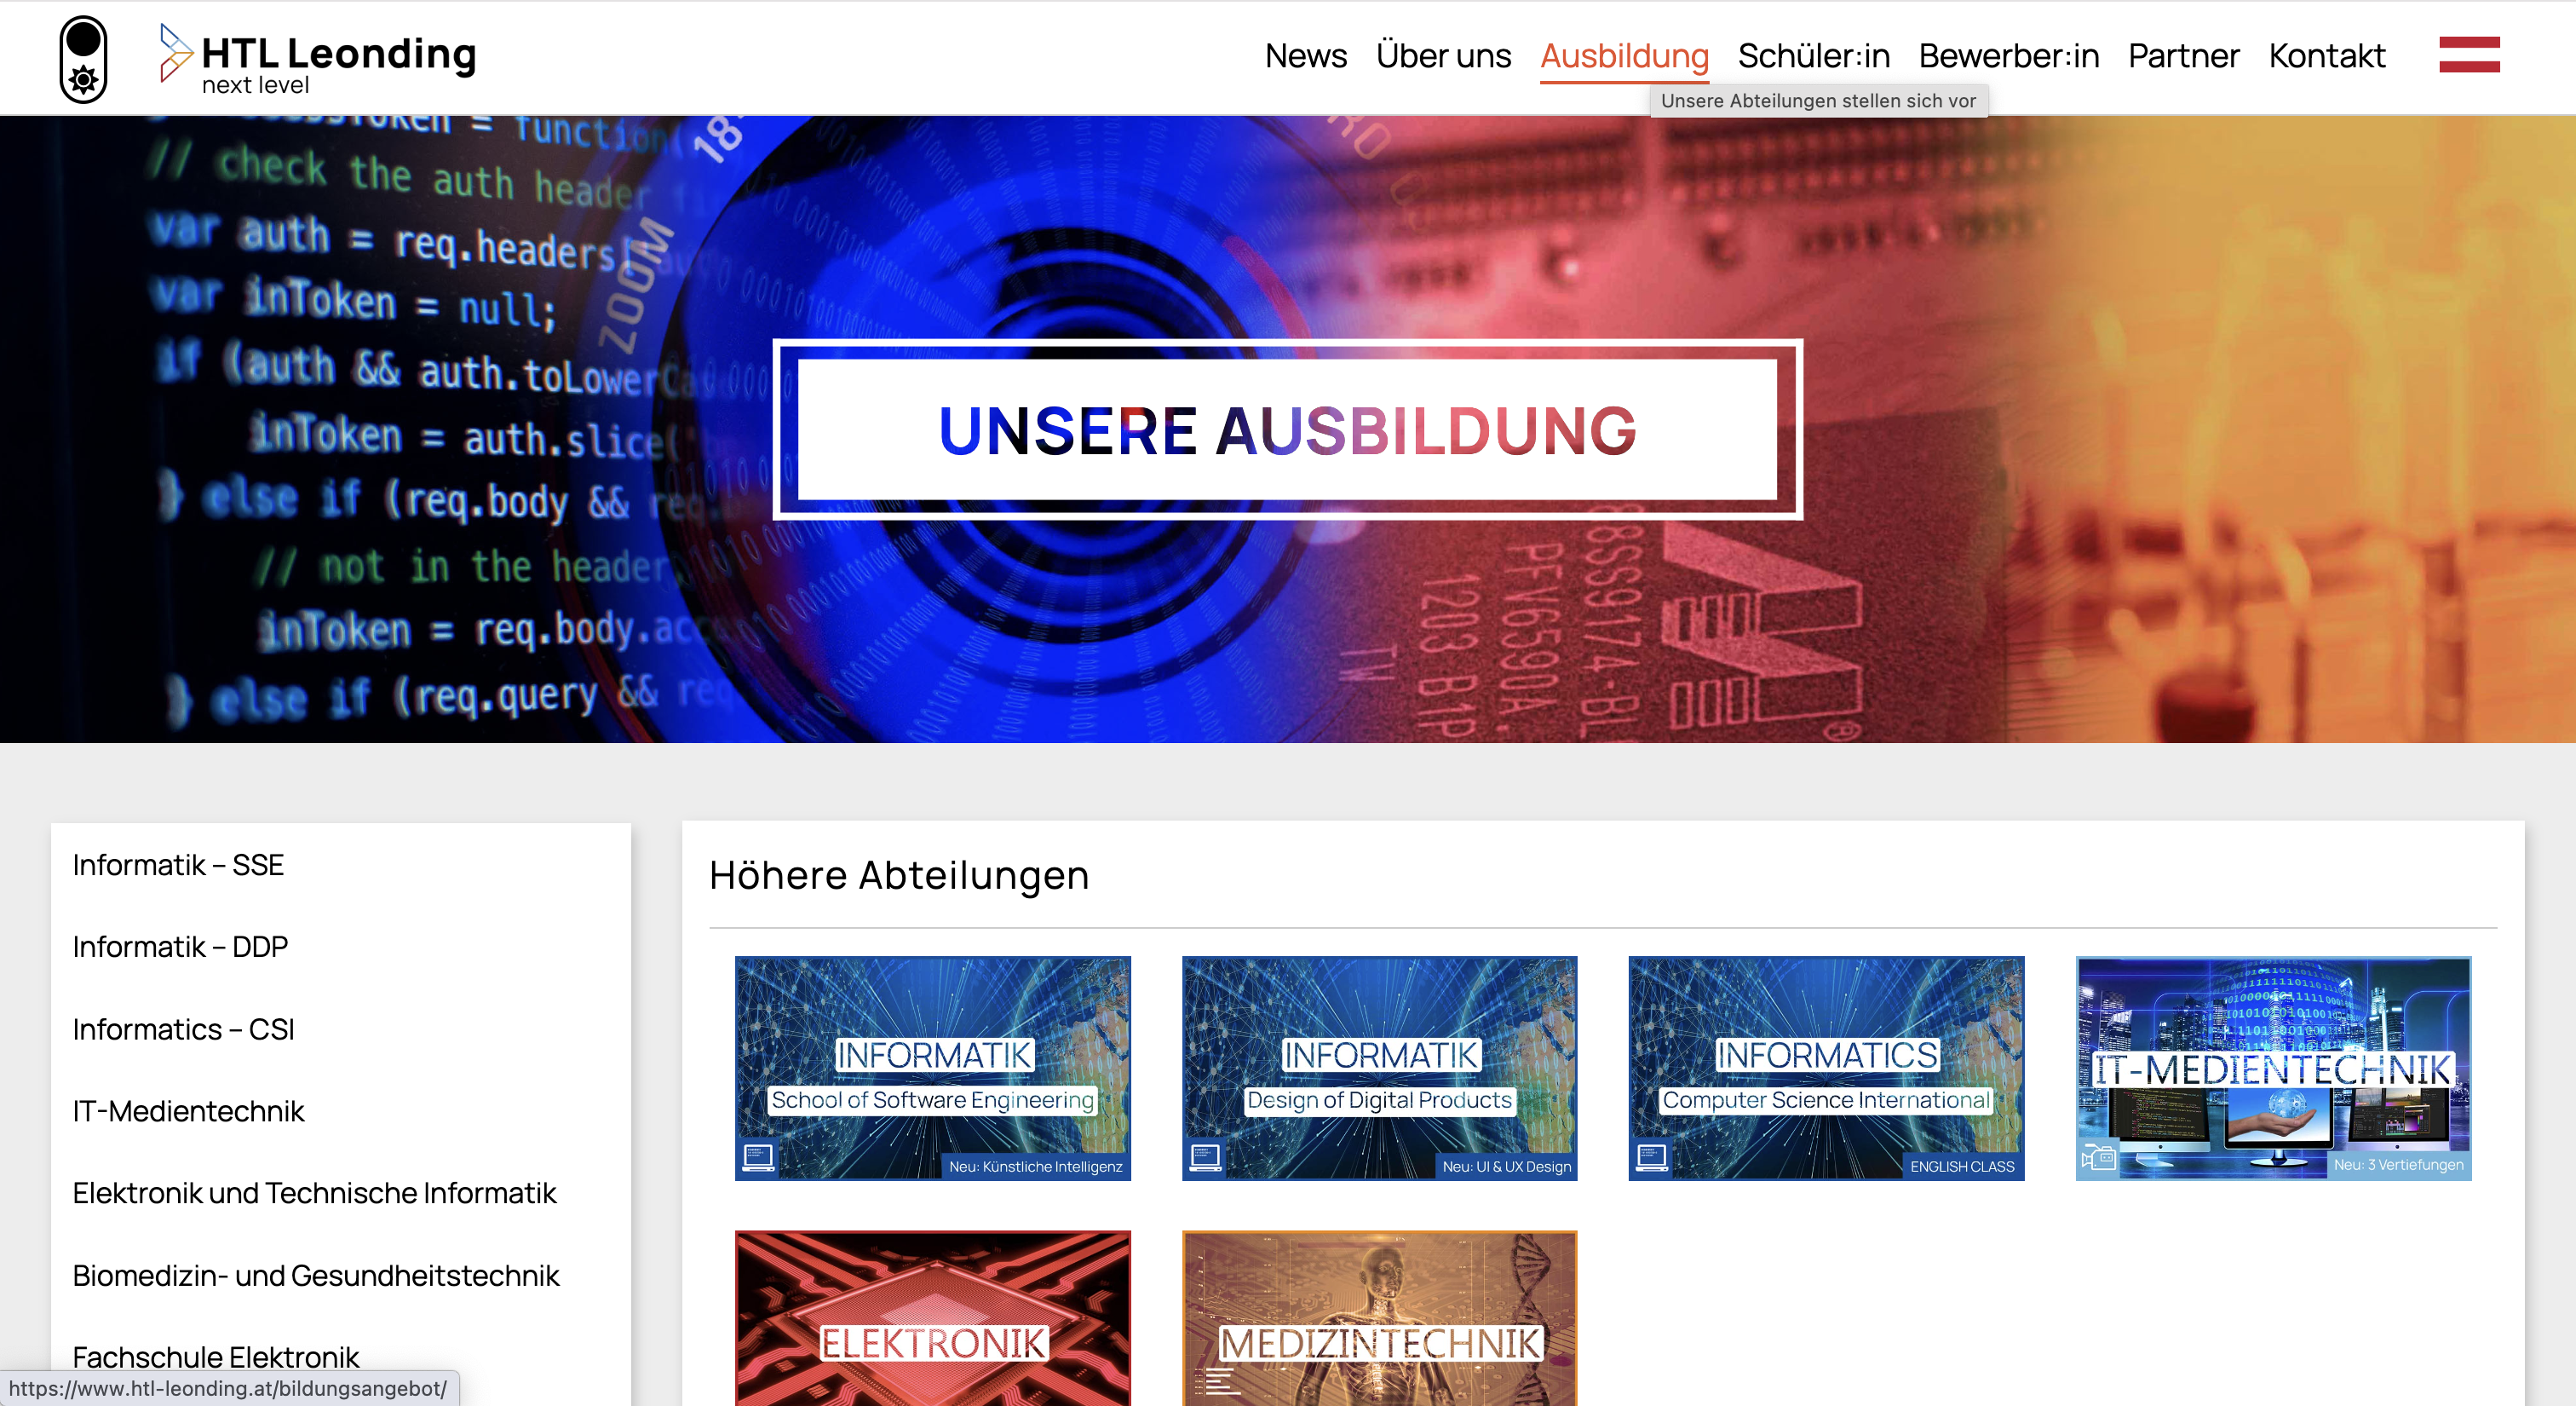
\includegraphics[width=\linewidth]{pics/alt-ausbildung.png}
      \caption{alte Ausbildungsseite}
      \label{fig:impl:alt:ausbildung}
   \end{minipage}
   \hspace{.05\linewidth}
   \begin{minipage}[b]{.4\linewidth}
      \includegraphics[width=\linewidth]{pics/neu-ausbildung.png}
      \caption{neue Ausbildungsseite}
      \label{fig:impl:neu:ausbildung}
   \end{minipage}
\end{figure}


\subsection{Bewerbung}
\setauthor{Angerer Mona}

Die Unterseite, die Bewerberinnen und deren Elternteile über den Anmeldeprozess informiert, ist eine der wichtigsten Seiten auf 
jeder Schulwebsite. Um sicherzustellen, dass diese Seite effektiv und benutzerfreundlich ist, wurde das Design sorgfältig ausgewählt. 
Ein zeitlicher Ablauf, der es den Benutzern ermöglicht, sich horizontal durchzubewegen, wurde als optimale Lösung gewählt.

Der Zeitstrahl ist mit nummerierten Schritten ausgestattet, um den Bewerbungsprozess transparent und leicht verständlich zu machen. 
Dies ermöglicht es allen Benutzern, egal ob SchülerInnen, BewerberInnen oder Eltern, schnell zu erfassen, wie der Vorgang der 
Bewerbung abläuft. Von der Informationsbeschaffung über die Einschreibung bis hin zur Bestätigung des Anmeldeprozesses werden alle Schritte 
klar und übersichtlich dargestellt.

Zusätzlich zu diesem Zeitstrahl findet man ein umfassendes FAQ (Häufig gestellte Fragen), das Antworten auf mögliche Fragen bezüglich der 
Wahl der Abteilung, benötigtem Notendurchschnitt oder dem genauen Ablauf der Anmeldung bietet. Dieses FAQ ist eine wertvolle Ressource 
für Bewerberinnen und ihre Elternteile, die möglicherweise Unsicherheiten oder Fragen bezüglich des Anmeldeprozesses haben. Es bietet 
klare und präzise Informationen, die dazu beitragen, potenzielle Probleme zu lösen und den Bewerbungsprozess reibungslos zu gestalten.

\begin{figure}
   \begin{minipage}[b]{.4\linewidth} 
      \includegraphics[width=\linewidth]{pics/alt-bewerbung.png}
      \caption{alte Bewerbungsseite}
      \label{fig:impl:alt:bewerbung}
   \end{minipage}
   \hspace{.05\linewidth}
   \begin{minipage}[b]{.4\linewidth}
      \includegraphics[width=\linewidth]{pics/neu-bewerbung.png}
      \caption{neue Bewerbungsseite}
      \label{fig:impl:neu:bewerbung}
   \end{minipage}
\end{figure}

\subsection{Kontakt}
\setauthor{Angerer Mona}

Die Unterseite, die sämtliche Kontakte der HTL Leonding auflistet, wurde sorgfältig gestaltet, um eine optimale Benutzererfahrung zu gewährleisten. Ein Großteil der Seite besteht aus horizontalen Scrollanimationen und Tabellen, die dazu dienen, die Informationen und Kontaktdaten übersichtlich zu strukturieren. Dieser Ansatz ermöglicht es den Besuchern, schnell und einfach durch die verschiedenen Kontakte zu navigieren, 
ohne von einer übermäßigen Menge an Text oder Bildern überwältigt zu werden.

Aufgrund der Länge der Seite wurde eine spezielle Navigationsstruktur implementiert, die es den Benutzern ermöglicht,
 direkt zu den relevanten Abschnitten zu springen, ohne lange scrollen zu müssen. Direkt unter dem Bannerbild mit der Überschrift 
 sind Links platziert, die die Benutzer direkt zu den gewünschten Inhalten führen. Diese Links sind strategisch positioniert, 
 um eine schnelle Navigation zu ermöglichen und sicherzustellen, dass die Benutzer mühelos finden, wonach sie suchen.

Die Verwendung von horizontalen Scrollanimationen verleiht der Seite Dynamik und Interaktivität, während gleichzeitig 
Platz gespart wird. Durch das horizontale Scrollen können Benutzer eine große Menge an Informationen auf kleinem Raum anzeigen, ohne
 die Seite zu überladen. Die Tabellen werden verwendet, um die Kontaktdaten in einer übersichtlichen und leicht verständlichen Form 
 darzustellen, was die Navigation erleichtert und sicherstellt, dass die Informationen schnell gefunden werden können.

 \begin{figure}
   \begin{minipage}[b]{.4\linewidth} 
      \includegraphics[width=\linewidth]{pics/alt-kontakt.png}
      \caption{alte Kontaktseite}
      \label{fig:impl:alt:kontakt}
   \end{minipage}
   \hspace{.05\linewidth}
   \begin{minipage}[b]{.4\linewidth}
      \includegraphics[width=\linewidth]{pics/neu-kontakt.png}
      \caption{neue Kontaktseite}
      \label{fig:impl:neu:kontakt}
   \end{minipage}
\end{figure}


\subsection{Schüler:innen}
\setauthor{Angerer Mona}

Anders als auf der bisherigen Website befindet sich der Menupunkt 'Schüler:innen' nicht mehr mit den anderen Links gesammelt im Menu, sondern 
ist nun auf der rechten Bildschirmseite platziert. Dies soll an das Einloggen oder die Profileinstellungne errinnern und so etwas Spannung in den Header
bringen und das Gefühl übermitteln, auf dieser Seite persönliche Informationen zu finden. Denn anders als bisher ist die Schüler:innen-Seite nicht mehr 
voller Links und organisatorischen Informationen gespickt, sondern zeigt das außerschulische Angebot, die Supportmöglichkeiten die den SchülerInnen
der HTL geboten wird und Fotos aller Schulklassen, um einen Einblick und ein Gefühl für die Stimmung in den Schulklassen zu erlangen.

\begin{figure}
   \begin{minipage}[b]{.4\linewidth} 
      \includegraphics[width=\linewidth]{pics/alt-schüler.png}
      \caption{alte Schüler:innenseite}
      \label{fig:impl:alt:kontakt}
   \end{minipage}
   \hspace{.05\linewidth}
   \begin{minipage}[b]{.4\linewidth}
      \includegraphics[width=\linewidth]{pics/neu-schüler.png}
      \caption{neue Schüler:innenseite}
      \label{fig:impl:neu:kontakt}
   \end{minipage}
\end{figure}


\section{Mobile Design}
\setauthor{Angerer Mona}

Aufgrund der begrenzten Bildschirmgröße und der unterschiedlichen Interaktionsmöglichkeiten auf mobilen Geräten im Vergleich zu 
Computern ist es entscheidend, das Design einer Website oder einer Anwendung für mobile Geräte anzupassen, um sicherzustellen, 
dass Benutzer eine optimale Erfahrung haben, unabhängig davon, welches Gerät sie verwenden.
Es muss sorgfältig darüber nachgedacht werden, welche Inhalte und Funktionen auf mobilen Geräten priorisiert werden sollen. Es müssen Elemente neu angeordnet,
 gestapelt oder zusammengefasst werden, um sicherzustellen, dass der Bildschirm nicht überladen wird und Benutzer leicht navigieren können.
Auch die Art und Weise, wie Benutzer mit mobilen Geräten interagieren, unterscheidet sich oft von der Interaktion mit Desktop-Computern. 
 Zum Beispiel verwenden Benutzer auf mobilen Geräten häufig Touchgesten wie Tippen, Wischen und Ziehen, während sie auf Desktops Mauszeiger 
 und Tastatureingaben verwenden. Auch in diesem Aspekt muss die Oberfläche für die mobile Version angepasst werden.
Die Leistung ist auf mobilen Geräten ebenfalls oft eine größere Herausforderung als auf Desktops, insbesondere in Bezug auf Ladezeiten 
und Ressourcenverbrauch. Daher muss darauf geachtet werden, dass das mobile Design optimiert ist, um eine schnelle 
Ladezeit und eine reibungslose Benutzererfahrung sicherzustellen. 

In Betrachtung dieser vorzunehmenden Anpassungen weichen im mobile Design einige Elemente von der Desktopversion ab.
Beispielsweise gibt es keine Startanimation (Siehe Abbildung \ref{fig:impl:mobile:start}), sondern die aktuellen Newsbeiträge werden direkt zum durchtippen angezeigt.
Auch fallen aufgrund Platzmangels die Schrägen in Headerbildern weg (Siehe Abbildung \ref{fig:impl:mobile:ausbildung}) und die Unterseiten sind in einem Burgermenu vereint. 


\begin{figure}
   \begin{minipage}[b]{.4\linewidth} 
      \includegraphics[width=\linewidth]{pics/start mobile.png}
      \caption{Startseite auf mobile Gerät}
      \label{fig:impl:mobile:start}
   \end{minipage}
   \hspace{.05\linewidth}
   \begin{minipage}[b]{.4\linewidth}
      \includegraphics[width=\linewidth]{pics/ausbildung mobile.png}
      \caption{Ausbildungsseite auf mobile Gerät}
      \label{fig:impl:mobile:ausbildung}
   \end{minipage}
\end{figure}